\documentclass[conference]{IEEEtran}
\usepackage{times}

% numbers option provides compact numerical references in the text. 
\usepackage[numbers]{natbib}
\usepackage{multicol}

\usepackage{caption}
\usepackage{subcaption}
\usepackage{times}
\usepackage{algorithm,algpseudocode}
\usepackage{tensor}
\usepackage{amsbsy}
\usepackage{optidef}
\usepackage{amsthm}
% numbers option provides compact numerical references in the text. 
%\usepackage[numbers]{natbib}
\usepackage{multicol}
\usepackage[bookmarks=true,draft]{hyperref}
\usepackage{graphicx}
\usepackage{array}
\usepackage{makecell}
\usepackage[utf8x]{inputenc}
\usepackage{amsmath}
\usepackage{amssymb}
\usepackage{cancel}
\usepackage{tikz}
\usetikzlibrary{bayesnet}
\newcommand{\me}{ \mathrm{e}}
\newcommand{\bx}{ \mathbf x }
\newcommand{\bu}{ \mathbf u }

\newcommand{\bA}{ \mathbf A }
\newcommand{\bB}{ \mathbf B }
\newcommand{\bQ}{ \mathbf Q }
\newcommand{\bR}{ \mathbf R }
\DeclareMathOperator*{\argmin}{arg\,min}
\usepackage{needspace}
\usepackage{color}
\usepackage{empheq}
\usepackage{stfloats}
%\usepackage{cite}
\usepackage{verbatim}
\usepackage{url}

\newtheorem{theorem}{Theorem}[section]
\newtheorem{corollary}{Corollary}[theorem]
\newtheorem{lemma}[theorem]{Lemma}
\makeatletter
\newcommand\footnoteref[1]{\protected@xdef\@thefnmark{\ref{#1}}\@footnotemark}
\makeatother


\begin{document}
%	\title{Fast Proximal Gauss-Newton Method for Real-time Constrained Nonlinear Model Predictive Control }
%	\title{Real-Time Constrained Nonlinear Model Predictive Control for Dynamic Legged Locomotion by Using Fast Proximal Gauss-Newton Method}
	\title{Real-Time Constrained Nonlinear Model Predictive Control for Dynamic Legged Locomotion}
	\author{Joon-Ha Kim, Seungwoo Hong, Hae-Won Park}
	\maketitle

\begin{abstract}
	 In this paper, we present a novel constrained nonlinear model predictive control framework for legged locomotion. We formulate the orientation error as in the manifold, and derive all necessary derivatives for the gradient and Gauss-Newton Hessian approximation. Furthermore, we extend our previous work to calculate Gauss-Newton Hessian approximation of orientation error in the objective function efficiently. Thanks to the fast nonlinear programming solver introduced in our previous work, we can implement various dynamic legged locomotion in real-time manner. An efficient algorithm to calculate Gauss-Newton Hessian approximation is newly proposed which reduces overall computational time of Gauss-Newton algorithm significantly. We tested the proposed method on a number of benchmark dynamic motion planning problems including nonlinear model predictive control of quadrupedal robots with twelve states and twelve control inputs. The combined framework offers reliable and robust performance on all the tested problems, demonstrating its capability to control a wide range of nonlinear dynamic systems.
	
%	This paper presents a novel trajectory optimization method for nonlinear model predictive control. The method solves an optimal control problem of discrete-time nonlinear dynamic systems with input constraints.  To accommodate input constraints, this method combines  Gauss-Newton algorithm for nonlinear least squares problem with a proximal mapping. An efficient algorithm to calculate Gauss-Newton Hessian approximation is newly proposed which reduces overall computational time of Gauss-Newton algorithm significantly. We tested the proposed method on a number of benchmark dynamic motion planning problems including nonlinear model predictive control of quadrupedal robots with twelve states and twelve control inputs. The combined framework offers reliable and robust performance on all the tested problems, demonstrating its capability to control a wide range of nonlinear dynamic systems.
	
	%This paper presents a novel trajectory optimization method for nonlinear model predictive control. The method solves an optimal control problem of discrete-time nonlinear dynamic systems with input constraints.  To accommodate input constraints, this method combines  Gauss-Newton algorithm for nonlinear least squares problem with a proximal mapping. An efficient algorithm to calculate Gauss-Newton Hessian approximation is newly proposed which reduces overall computational time of Gauss-Newton algorithm significantly. We tested the proposed method on a number of benchmark dynamic motion planning problems including nonlinear model predictive control of quadrupedal robots with twelve states and twelve control inputs. The combined framework offers reliable and robust performance on all the tested problems, demonstrating its capability to control a wide range of nonlinear dynamic systems.
	
	%This paper presents a planning framework for jumping over obstacles with quadruped robots. The framework accomplishes planning via a structured predictive control strategy that combines the use of heterogeneous simplified models over different prediction time scales. A receding multi-horizon predictive controller coordinates the approach before the jump using a kinematic point-mass model. Consideration of the optimal value function over different planning horizons enables the system to select an appropriate number of steps to take before jumping. The jumping motion is then tailored to the sensed obstacle by solving a nonlinear trajectory optimization problem. The solution of this problem online is enabled by exploiting the analyticity of the flow map for a planar bounding template model under polynomial inputs. 
	%By planning with this combination of models, MIT Cheetah 2 is shown to autonomously jump over obstacles up to 40 cm in height during high-speed bounding. Untethered results showcase the ability of the method to automatically adapt to obstacles of different heights and placements in a single trial. 
	
	%We propose new control system components, layered on top of a low-level running controller, which actively modify the approach to a sensed obstacle and select stance force profiles as required to clear it. The approach controller enables the quadruped to end in a preferable location relative to the obstacle just before the jump. This multi-step gait planning  is formulated as a multiple-horizon model predictive control problem and solved at each step through quadratic programming. Ground reaction force profiles to execute the running jump are selected through constrained nonlinear optimization on a simplified model of the robot that possesses polynomial dynamics. Exploiting this structure of these simplified dynamics, the presented method greatly accelerates the computation of otherwise costly function and constraint evaluations that are required during optimization. With these considerations, the new algorithms allow for online planning that is critical for reliable response to unexpected situations. Experimental results, for a stand-alone quadruped with on-board power and computation, show the viability of this approach, and represent important steps towards broader dynamic maneuverability in experimental machines.
\end{abstract}

\section{Introduction}
%Due to recent advances in computer hardware systems and optimization algorithms, model predictive control (MPC) has become more plausible control design options for complex dynamic systems~\cite{8594448,8276298,8793669}. In nonlinear MPC design, a control input is chosen as the solution of the trajectory optimization problem of nonlinear systems at every sampling time. Challenges in application of nonlinear MPC arise from limited computation time which is required for real-time implementation and various inequality and equality constraints due to hardware limitation and environments. In this point of view, many algorithms are proposed to solve this trajectory optimization problem efficiently and robustly. 
%
%One widely used method for trajectory optimization is direct methods that formulate  optimal control problems into the finite-sized optimization problems treating both states and controls as decision variables~\cite{von1993numerical,patterson2014gpops,8202230}. For nonlinear MPC, this process results in nonlinear programming problems which are solved using general-purpose nonlinear programming (NLP) solvers~\cite{wachter2006implementation,gill2002snopt}. Although it is very easy and simple to apply this method to general optimal control problems, the formulated optimization problem easily become a very large optimization problem for high Degrees of Freedom (DoF) dynamic systems and its performance heavily rely on that of NLP solvers.  %In spite of its simplicity and easiness of application in general optimal control problems, this algorithm hardly utilizes the structure of the optimal control problem, and heavily rely on the performance of NLP solvers.
%
%On the other hand, indirect approaches only parameterize controls as decision variables and states are obtained by propagating initial states through a dynamic equation. Differential Dynamic Programming (DDP) is one of such approaches that locally search around current controls and states utilizing derivative information of dynamics and cost. Since DDP decompose a large optimization problem into small sub-problems, it is better fitted to the applications where fast computation is critical such as nonlinear MPC. 
%However, incorporating constraints is not straightforward in this method, and many modifacations have been proposed rooting back to studies in~\cite{1101692,doi:10.1029/WR015i005p01017} using active-set like algorithms. Originating from these works, more recently, the works in~\cite{6907001} proposes control-limited DDP algorithm that can handle box constraints on control inputs and ~\cite{xie2017differential} proposes algorithm with an ability of handling also state constraints. Augmented Lagrangian  (AL) method is another popular approach incorporating inequality constraints, and recently, a number of algorithms proposed in~\cite{howell2019altro,lantoine2012hybrid} uses it.   
%
%%Before application of MPC, controller design for complex dynamic systems relied on heuristically designed control pricinples based upon simplified representation of dynamic models.    
%
%In this paper, we present a trajectory optimization framework for input constrained nonlinear model predictive control using Gauss-Newton algorithms combined with proximal operators of an indicator function. Instead of using Hessian, the Gauss-Newton algorithm uses Gauss-Newton Hessian approximation to obtain the line search direction. Unlike other approaches, to handle control input constraints, a proximal operator is applied to the line search direction. A rate of convergence of the algorithm can be improved by scaling a proximal operator with Gauss-Newton Hessian approximation. For linear input inequality constraints, an output of this scaled proximal operator can be obtained by solving simple quadratic programming (QP) problems\footnote{For a convex non-empty set, this problem becomes convex nonlinear programming}.%, hence computationally efficient process using state-of-the-art QP solvers.  
%
%To scale the proximal operator, we need to explicitly obtain the Gauss-Newton Hessian approximation matrix of the nonlinear optimal problem which is computationally burdensome. Modern automatic differentiation (AD) tools can be utilized to construct such matrix, but we found that code generation and library building of Gauss-Newton Hessian approximation matrix take a quite amount of time for long horizon MPC problems of dynamic systems. For example, it took 41 minutes for code generation and building of Gauss-Newton Hessian approximation matrix for simple cart-pole optimal control problem with a horizon of $50$ using CppAD~\cite{bell2012cppad} and CppADCodeGen compiled with the Clang compiler~\cite{lattner2008llvm}. To solve this problem, we present a novel algorithm to efficiently calculate Gauss-Newton Hessian approximation similar to the Composite-Rigid-Body algorithm for a joint-space inertia matrix. This similarity is based on the relation between the forward dynamics problem and the linear quadratic optimal control problem established by Gauss's principle~\cite{wieber2005some,vereshchagin1974computer}. This new algorithm reduced computational complexity of Gauss-Newton Hessian approximation from $\mathcal{O}(N^3)$ to $\mathcal{O}(N^2)$ with respect to the horizon length $N$.
Animals in real world are capable of traversing in a precarious environment. For instance, an ibex can scale up nearly vertical cliffs by controlling and coordinating their dexterous hooves. Those incredible phenomena in nature motivates the realm of legged robotics to mimick the highly dynamic locomotion that animals can achieve. However, control sophisticated dynamic locomotion for legged robots is a demanding problem due to the nonlinear dynamics and the underactuation of the floating base that can only be controlled indirectly by the internal motion of the robot and the external wrenches exerted on the robot. This difficulty is further complicated by the constraints such as friction cone constraints that should be imposed on those external wrenches to avoid slip motion occured. One of the promising approaches that can solve this kind of problem is an optimization based approach that has shown remarkable performance recently.



The application of MPC on legged robots can be classified into two large groups, convex and nonconvex MPC approaches. Applications of convex MPC from humanoids~\cite{wieber2006trajectory},~\cite{diedam2008online},~\cite{herdt2010online},

In general, those two approaches impose a tradeoff between the model accuracy and computational efficiency. On one hand, convex MPC approaches enable a fast calculation, but their accuracy is deteriorated by approximation of nonlinear dynamics. On the other hand, nonconvex MPC approaches, based on nonlinear optimization, are accurate, but computationally demanding. 

Since computational efficiency is important for controlling dynamic legged locomotion, many researchers choose to approximate the nonlinear dynamics as affine one. Since the convex MPC can be implemented in a real-time manner. 

Linear inverted pendulum model (LIPM), centroidal dynamics, single rigid body dynamics.

Single rigid body dynamics offers a compromise between accuracy and efficiency; however, it is not clear how to parameterize the orientation to perform dynamic maneuvers such a back-flip and wall-climbing motions. 

The above researches adopted Euler angles as the global parameterization for rotations. Using Euler angles as parameterization for rotations is not properly invariant under the action of rigid transformations~\cite{forster2016manifold}. Moreover, Euler angles are known to have singularities. In this study, we address the manifold structure of the rotation group $\mathrm{SO(3)}$. 

In this study, we show that it is possible to overcome this tradeoff. First, we parameterize the orientation error in tangent space of manifold. Second, we propose a novel MPC framework that enables real-time calculation of optimal solutions by using a novel NLP solvers. 

The first step toward this goal is the development of all necessary Jacobians for the optimization. Furthermore, we are able to derive all necessary Jacobians in analytic form: specifically, we report the analytic Jacobians of the sigle rigid body dynamics. Compared with local parameterization or direct linearization on manifold, our method is ...\begin{flushleft}
	
\end{flushleft}

% !TEX root = Estimation_Junny.tex

\section{State and Measurement Definition} \label{State_Measurement}
%In this work, we formulate legged locomotion control problem in terms of the MPC problem. In our model, the MPC leads to a nonlinear programming due to the rotation matrix living on smooth manifolds. This motivates us to use the NMPC approach.
%In this work, we formulate legged locomotion control problem in terms of the NMPC problem. This is due to the rotation matrix, which lives on smooth manifolds, in our model. Therefore, this render us to use a nonlinear programming to solve the NMPC problem.
In this section, we define the state and measurement model of legged robot state estimation.
%Thus, a novel NMPC framework will be introduced in this section. 
Consider an optimal control problem of discrete-time deterministic system that consists of states $\mathbf{x}_{k} \in \mathbb{R}^{n}$ and control inputs $\mathbf{u}_{k} \in \mathbb{R}^{m}$ with a finite time horizon ${N}$. This optimal control problem consists of three parts. % ;namely, an objective function, dynamics of the system, and contraints of control inputs.



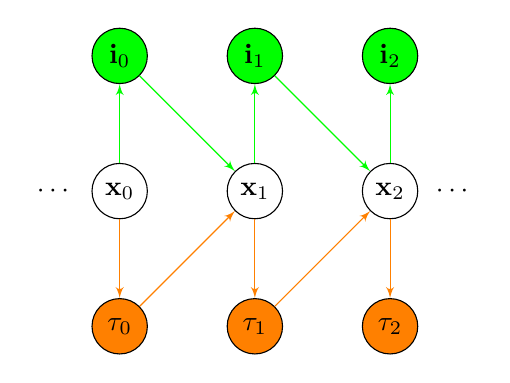
\begin{tikzpicture}
[node distance=19mm,auto,>=latex',
box/.style={draw, minimum size=0.6cm},
short/.style={node distance=14mm}]
\node[draw = none] (start) {$\cdots$};

\node[latent, right=0.1 of start] (x0) {$\mathbf{x}_0$};

\node[obs,fill=green, above=1.0 of x0] (i0) {$\mathbf{i}_0$};
\node[obs,fill=orange, below=1.0 of x0] (tau0) {$\mathbf{\tau}_0$};
\edge[color=green] {x0} {i0};
\edge[color=orange] {x0} {tau0};

\node[latent, right=1.0 of x0] (x1) {$\mathbf{x}_1$};

\edge[color=green] {i0} {x1};
\edge[color=orange] {tau0} {x1};

\node[obs,fill=green, above=1.0 of x1] (i1) {$\mathbf{i}_1$};
\node[obs,fill=orange, below=1.0 of x1] (tau1) {$\mathbf{\tau}_1$};
\edge[color=green] {x1} {i1};
\edge[color=orange] {x1} {tau1};

\node[latent, right=1.0 of x1] (x2) {$\mathbf{x}_2$};

\edge[color=green] {i1} {x2};
\edge[color=orange] {tau1} {x2};

\node[obs,fill=green, above=1.0 of x2] (i2) {$\mathbf{i}_2$};
\node[obs,fill=orange, below=1.0 of x2] (tau2) {$\mathbf{\tau}_2$};
\edge[color=green] {x2} {i2};
\edge[color=orange] {x2} {tau2};

\node[right=0.1 of x2] (end) {$\cdots$};
%\node[obs]                    (k)   {$\mathbf{x}_0$}; %
%\node[latent, right=2 of k]   (l)   {$\lambda$}; %
%\node[right = 0.7 of k] (dots) {$\cdots$};
%\edge[draw=none] {k} {l}
\end{tikzpicture}

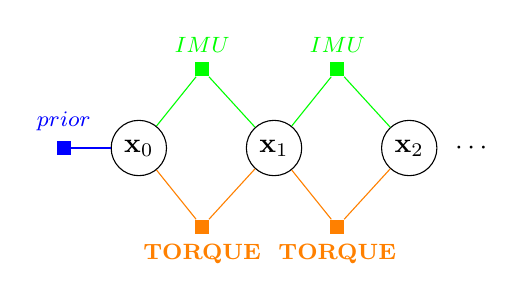
\begin{tikzpicture}
[node distance=19mm,auto,>=latex',
box/.style={draw, minimum size=0.6cm},
short/.style={node distance=14mm}]
\factor[color=blue] {start} {$ \textcolor{blue}{prior}$} {} {};

\node[latent, right=0.5 of start] (x0) {$\mathbf{x}_0$};
\edge[-,color=blue] {start} {x0};
\factor[color=green, right=0.35 of x0,yshift=1.0cm] {i0} {$ \textcolor{green}{IMU}$} {} {};
\factor[color=orange, right=0.35 of x0,yshift=-1.0cm, label=below:$ \textcolor{orange}{\mathbf{TORQUE}}$] {tau0} {} {} {};
\edge[-,color=green] {x0} {i0};
\edge[-,color=orange] {x0} {tau0};

\node[latent, right=1.0 of x0] (x1) {$\mathbf{x}_1$};

\edge[-,color=green] {i0} {x1};
\edge[-,color=orange] {tau0} {x1};

\factor[color=green, right=0.35 of x1,yshift=1.0cm] {i1} {$ \textcolor{green}{IMU}$} {} {};
\factor[color=orange, right=0.35 of x1,yshift=-1.0cm, label=below:$ \textcolor{orange}{\mathbf{TORQUE}}$] {tau1} {} {} {};
\edge[-,color=green] {x1} {i1};
\edge[-,color=orange] {x1} {tau1};

\node[latent, right=1.0 of x1] (x2) {$\mathbf{x}_2$};

\edge[-,color=green] {i1} {x2};
\edge[-,color=orange] {tau1} {x2};



\node[right=0.1 of x2] (end) {$\cdots$};
\end{tikzpicture}

% !TEX root = Estimation_Junny.tex

%\subsection{Preliminaries and Theoretical Background}
%This section recalls some properties of Lie group and Lie Algebra that are necessary for the derivations proposed in the next section. 

% 이 논문은 Legged robot을 제어하기 위한 reference가 주어졌을 때, Legged robot의 optimal GRF를 계산하여 torque로 환산한 후 로봇의 제어 입력을 넣는다. 이를 구현하기 위해 legged robot의 dynamic locomotion 제어 문제를 optimal control 문제의 일종인 model predictive control 문제로 접근하였다. 그러나 Legged robot의 dynamics를 multi-link rigid body로 가정하면 문제가 매우 복잡해지고 계산량이 방대해지므로 본 논문에서는 이러한 복잡한 dynamics를 single rigid body dynamics (SRB)로 가정하고 접근하였다. 비록 SRB는 multi-link dynamics에 비해 고려해야할 state와 control input이 적지만, 여전히 nonlinearity 성질을 갖고 있기 때문에 nonlinear model predictive control을 사용하게 되었다. 

\section{asdfasdfadsf} \label{asdfasdfasdfasdf}
%In this work, we formulate legged locomotion control problem in terms of the MPC problem. In our model, the MPC leads to a nonlinear programming due to the rotation matrix living on smooth manifolds. This motivates us to use the NMPC approach.
%In this work, we formulate legged locomotion control problem in terms of the NMPC problem. This is due to the rotation matrix, which lives on smooth manifolds, in our model. Therefore, this render us to use a nonlinear programming to solve the NMPC problem.
In this section, we define the state and measurement model of legged robot state estimation.
%Thus, a novel NMPC framework will be introduced in this section. 
Consider an optimal control problem of discrete-time deterministic system that consists of states $\mathbf{x}_{k} \in \mathbb{R}^{n}$ and control inputs $\mathbf{u}_{k} \in \mathbb{R}^{m}$ with a finite time horizon ${N}$. This optimal control problem consists of three parts. % ;namely, an objective function, dynamics of the system, and contraints of control inputs.
The first part is a nonlinear model that describes the dynamics of the system given as
\begin{align}
\label{eq:NMPC_dyn}
\mathbf{x}_{k+1} = \mathbf{f}(\mathbf{x}_{k},\mathbf{u}_{k})
\end{align}
%Let $\mathbf{X}_{k}$ and $\mathbf{U}_{k}$ represent the collection of all states and control inputs up to time step $k$
%\begin{align}
%\label{eq:Xs}
%\mathbf{X}_{k} &\coloneqq \{ \mathbf{x}_{1},...,\mathbf{x}_{\mathrm{k}} \}
%\end{align}
where ${k} \in \{0,1,\cdots,{N}\}$, and $\mathbf{x}_{0}$ is a given initial state. The second part is the objective function ${J}$, which is the sum of weighted deviations of the states and control inputs from a set of desired quantities in a least-squares sense over the entire time horizon considered 
\begin{align}
\label{eq:NMPC_objfcn1}
J(\mathbf{x},\mathbf{u}) &= \sum_{k=1}^{N}\frac{1}{2}\|\mathbf{r}_{\mathbf{x}_{k}}\|^2_{\mathbf{\widetilde{Q}}_k} + \sum_{k=0}^{N-1}\frac{1}{2}\|\mathbf{r}_{\mathbf{u}_{k}}\|^2_{\mathbf{\widetilde{R}}_k}
\end{align}
%$\mathbf{x}=\{\mathbf{x}_{1},\mathbf{x}_{2},...,\mathbf{x}_{N}\}$, $\mathbf{u}=\{\mathbf{u}_{0},\mathbf{u}_{1},...,\mathbf{u}_{N-1}\}$,
%$\mathbf{r}_{\mathbf{x}_{k}} = \mathbf{r}(\mathbf{x}_{k})$
where $\mathbf{r}_{\mathbf{x}_{k}} = \mathbf{h}(\mathbf{x}_{k})$ is a nonlinear residual error of state, and  $\mathbf{r}_{\mathbf{u}_{k}}=\mathbf{u}_{k}-\mathbf{u}^{d}_{k}$ is a linear residual error of control input at time step $k$, respectively; $\mathbf{\widetilde{Q}}_{k} \in \mathbb{S}^{n}_{++}$ and $\mathbf{\widetilde{R}}_{k} \in \mathbb{S}^{m}_{++}$ are the corresponding weight matrices. 

%\begin{align}
%\label{eq:NMPC_objfcn1}
%J(\mathbf{x},\mathbf{u}) &= \sum_{k=1}^{N}\frac{1}{2}\|\mathbf{r}_{\mathbf{x}_{k}}(\mathbf{x}_{k},\mathbf{x}^{d}_{k})\|^2_{\mathbf{\widetilde{Q}}_k} + \sum_{k=0}^{N-1}\frac{1}{2}\|\mathbf{r}_{\mathbf{u}_{k}}(\mathbf{u}_{k},\mathbf{u}^{d}_{k})\|^2_{\mathbf{\widetilde{R}}_k}
%\end{align}
%where $\mathbf{r}_{\mathbf{x}_{k}}(\mathbf{x}_{k},\mathbf{x}^{d}_{k})$ and $\mathbf{r}_{\mathbf{u}_{k}}(\mathbf{u}_{k},\mathbf{u}^{d}_{k})$ are the residual errors of state and control input at time step $k$; $\mathbf{\widetilde{Q}}_{k} \in \mathbb{S}^{n}_{++}$ and $\mathbf{\widetilde{R}}_{k} \in \mathbb{S}^{m}_{++}$ are the corresponding weight matrices. 
The final part contains constraints on control inputs that can be formulated as affine functions
\begin{align}
\label{eq:NMPC_constraint1}
\mathbf{A}_{k}\mathbf{u}_{k} &\leq \mathbf{b}_{k} \\
%\mathbf{A}\mathbf{u} &\leq \mathbf{b} \\
\label{eq:NMPC_constraint2}
\mathbf{C}_{k}\mathbf{u}_{k} &= \mathbf{d}_{k}
%\mathbf{C}\mathbf{u} &= \mathbf{d}
\end{align}
%$\mathbf{x}=\{\mathbf{x}_{1},\cdots,\mathbf{x}_{\mathrm{N}}\}$
%$\mathbf{u}=\{\mathbf{u}_{0},\cdots,\mathbf{u}_{\mathrm{N-1}}\}$

Moreover, the decision variables can be parameterized with only control inputs $\mathbf{u}$ by representing the state variables $\mathbf{x}$ as a function of $\mathbf{u}$ using model dynamics~\eqref{eq:NMPC_dyn}.
%The state variables $\mathbf{x}$ can be eliminated from the decision variables by expressing them as a function of $\mathbf{u}$ using the model dynamics~\eqref{eq:NMPC_dyn}. 
For notational convenience, we define ${\mathbf{f}}_{\mathbf{u}_k}(\mathbf{x}):=\mathbf{f}(\mathbf{x}_k,\mathbf{u}_k)$ and the collection of control inputs and desired control inputs up to the time step $k-1$, $\mathbf{U}_k:=[\mathbf{u}_{0}^T,\cdots,\mathbf{u}_{k-1}^T]^T$ and $\mathbf{U}^d_k:=[{\mathbf{u}^d_{0}}^T,\cdots,{\mathbf{u}^d_{k-1}}^T]^T$. Then, the state $\mathbf{x}_k$ can be expressed as
\begin{align} \label{eq:NMPC_states_k}
\mathbf{x}_k = \boldsymbol{\phi}_k(\mathbf{U}_{k})=\mathbf{f}_{\mathbf{u}_{k-1}}\circ \mathbf{f}_{\mathbf{u}_{k-2}}\circ \cdots \circ \mathbf{f}_{\mathbf{u}_{0}}(\mathbf{x}_0)
\end{align}

%Rewriting the objective function~\eqref{eq:NMPC_objfcn1} using~\eqref{eq:NMPC_states_k} with $\mathbf{h}_{k}(\mathbf{x}):=\mathbf{h}(\mathbf{x}_{k})$ yields
Substituting~\eqref{eq:NMPC_states_k} into the objective function~\eqref{eq:NMPC_objfcn1} with $\mathbf{h}_{k}(\mathbf{x}):=\mathbf{h}(\mathbf{x}_{k})$ yields
\begin{align} \label{eq:NMPC_objfcn2}
J(\mathbf{U}_N) &= \sum_{k=1}^{N}\frac{1}{2}\|\mathbf{h}_{k}(\boldsymbol{\phi}_k(\mathbf{U}_{k}))\|^2_{\mathbf{\widetilde{Q}}_k} + \sum_{k=0}^{N-1}\frac{1}{2}\|\mathbf{u}_{k}-\mathbf{u}^{d}_{k}\|^2_{\mathbf{\widetilde{R}}_k}
\end{align}

With the objective function~\eqref{eq:NMPC_objfcn2}, the finite-horizon discrete-time optimal control problem becomes
\begin{mini}|s|
	{\mathbf{U}_{N}}{\sum_{k=1}^{N}\frac{1}{2}\|\mathbf{h}_{k}(\boldsymbol{\phi}_k(\mathbf{U}_{k}))\|^2_{\mathbf{\widetilde{Q}}_k} + \sum_{k=0}^{N-1}\frac{1}{2}\|\mathbf{u}_{k}-\mathbf{u}^{d}_{k}\|^2_{\mathbf{\widetilde{R}}_k}}
	{\label{eq:NMPC_OCP}}{}
	%	\addConstraint{ \mathbf{A}_{k} \mathbf{u}_{k} \leq \mathbf{b}_{k}, k=0,\cdots,N-1}
	%	\addConstraint{ \mathbf{C}_{k} \mathbf{u}_{k} = \mathbf{d}_{k}, k=0,\cdots,N-1}
	\addConstraint{ \mathbf{A}_{k} \mathbf{u}_{k} \leq \mathbf{b}_{k}, \quad {k} \in \{0,\cdots,{N-1}\}}
	\addConstraint{ \mathbf{C}_{k} \mathbf{u}_{k} = \mathbf{d}_{k}, \quad {k} \in \{0,\cdots,{N-1}\}}
\end{mini}
which is in the form of constrained nonlinear least-squares problem.

Application of the proximal Gauss-Newton algorithm to this problem requires calculating the gradient and Gauss-Newton Hessian approximation of the objective function.
The gradient of the objective function~\eqref{eq:NMPC_objfcn2} is given by
\begin{align}
\label{eq:J1}
\mathbf{J} =\sum^N_{k=1} \frac{\partial \boldsymbol{\phi}_k}{\partial \mathbf{U}_N}^{T} \mathbf{\widetilde{Q}}^{'}_{k} \mathbf{h}_{k}(\boldsymbol{\phi}_k(\mathbf{U}_{k})) + \boldsymbol{\Phi}_{\mathbf{\widetilde{R}}} (\mathbf{U}_N-\mathbf{U}^d_N)
\end{align}

%where $\mathbf{\widetilde{Q}}^{'}_{k} = (\frac{\partial \mathbf{h}_k}{\partial \mathbf{x}})^{T} \mathbf{\widetilde{Q}}_{k}$, and $\boldsymbol{\Phi}_{\mathbf{\widetilde{R}}}$ is a block diagonal matrix formed by $\rm{blkdiag}(\mathbf{\widetilde{R}}_0,\cdots,\mathbf{\widetilde{R}}_{N-1})$.
%Similarly, the Gauss-Newton Hessian approximation of the objective function~\eqref{eq:NMPC_objfcn2} is given by

%junny
where $\mathbf{\widetilde{Q}}^{'}_{k} = (\frac{\partial \mathbf{h}_k}{\partial \mathbf{x}})^{T} \mathbf{\widetilde{Q}}_{k}$, and $\boldsymbol{\Phi}_{\mathbf{\widetilde{R}}}$ is a block diagonal matrix formed with diagonal elements as $\{ \mathbf{\widetilde{R}}_0,\cdots,\mathbf{\widetilde{R}}_{N-1} \}$.
Similarly, the Gauss-Newton Hessian approximation of the objective function~\eqref{eq:NMPC_objfcn2} is given by


\begin{align}
\label{eq:H_GN1}
\mathbf{H}_{GN}=\sum_{k=1}^{N} \frac{\partial \boldsymbol{\phi}_k}{\partial \mathbf{U}_N}^{T} \mathbf{\widetilde{Q}}^{''}_k \frac{\partial \boldsymbol{\phi}_k}{\partial \mathbf{U}_N} + \boldsymbol{\Phi}_{\mathbf{\widetilde{R}}}
\end{align}
where $\mathbf{\widetilde{Q}}^{''}_{k} = (\frac{\partial \mathbf{h}_k}{\partial \mathbf{x}})^{T} \mathbf{\widetilde{Q}}_{k} (\frac{\partial \mathbf{h}_k}{\partial \mathbf{x}})$.

The first term of $\mathbf{J}$ and $\mathbf{H}_{GN}$ has $\frac{\partial \boldsymbol{\phi}_i}{\partial \mathbf{U}_N}=\begin{bmatrix}\frac{\partial \boldsymbol{\phi}_i}{\partial \mathbf{u}_0} & \cdots & \frac{\partial \boldsymbol{\phi}_i}{\partial \mathbf{u}_{N-1}} \end{bmatrix}\in \mathbb{R}^{n\times Nm}$ and $\frac{\partial \boldsymbol{\phi}_i}{\partial \mathbf{u}_j}$ is given by
\begin{align}
\label{eq:Phi}
\frac{\partial \boldsymbol{\phi}_i}{\partial \mathbf{u}_j}=
\boldsymbol{\pi}_{i,j}\frac{\partial \mathbf{f}_j}{\partial \mathbf{u}}
%\begin{cases}
%\frac{\partial \mathbf{f}_{i-k}}{\partial \mathbf{x}}\frac{\partial \mathbf{f}_{i-k-1}}{\partial \mathbf{x}} \cdots \frac{\partial %\mathbf{f}_{k+1}}{\partial \mathbf{x}} \frac{\partial \mathbf{f}_{k}}{\partial \mathbf{u}} & 1\leq k\leq i\\0 & i<k\leq N\end{cases}
\end{align}
where, 
\begin{align}
\boldsymbol{\pi}_{i,j}=\begin{cases} \prod_{k=j}^{i-2} \frac{\partial \mathbf{f}_{-k+j+i-1}}{\partial \mathbf{x}} & i\geq j+2\\\mathbf{I}^{n\times n} &i=j+1\\\mathbf{0}^{n\times n} & {\rm otherwise} \end{cases}
\end{align}
with $\frac{\partial \mathbf{f}_j}{\partial \mathbf{x}}:=\frac{\partial \mathbf{f}(\mathbf{x}_j,\mathbf{u}_j)}{\partial \mathbf{x}}$, $\frac{\partial \mathbf{f}_j}{\partial \mathbf{u}}:=\frac{\partial \mathbf{f}(\mathbf{x}_j,\mathbf{u}_j)}{\partial \mathbf{u}}$. \newline

%For an unconstrained optimization problem, a standard Gauss-Newton method can be used to find a solution for the next iteration efficiently. We will extend the standard Gauss-Newton method to constrained optimization problem to handle the constraints~\eqref{eq:NMPC_constraint1} and~\eqref{eq:NMPC_constraint2}. The details of formulating the legged locomotion problem as a NMPC structure and the extended Gauss-Newton method will be introduced in the following subsections.

The details of formulating the legged locomotion problem as a NMPC framework will be provided in \ref{Model_Dynamics}, \ref{Objective_Function}, \ref{Reference_Generation}, \ref{Constraints}, and all the Jacobians necessary to calculate the gradient and Gauss-Newton Hessian approximation of the objective function will be introduced in \ref{Jacobians}. 

%The details of how we choose optimization variables, objective function, equality constraints, and inequality constraints respectively will be introduced in the following subsections.
%The details of formulating the legged locomotion problem as a NMPC structure will be introduced in the following subsections.
%the state $\mathbf{x}$, control input $\mathbf{u}$, objective function ${J}$, equality constraints, and inequality constraints respectively will be introduced in the following sections.
%In the following subsections, we will provide the details 

\subsection{Model Dynamics} \label{Model_Dynamics}
%For a physically realizable motion, the dynamics of the robot should satisfy the Newton's and Euler's equation of motion; namely, the rate of linear momentum $\mathcal{P}$ and angular momentum $\mathcal{L}$ of the robot should comply with all the external wrenches applied to the robot. Consider a legged robot as a floating base sigle rigid body with point feet, then the equation of motion is given by 
%\begin{align}
%%\frac{d}{dt} \mathcal{P} &= \mathbf{f}_{ext} \\
%%\frac{d}{dt} \mathcal{L} &= \pmb{\tau}_{ext}
%%\frac{d}{dt} \mathcal{P} &= \mathbf{f}_{ext} = \sum_{i=1} \mathbf{f}_i + {m} \mathbf{g}\\
%%\frac{d}{dt} \mathcal{L} &= \pmb{\tau}_{ext} = \sum_{i=1} \mathbf{r}_i \times \mathbf{f}_{i}
%\frac{d}{dt} \mathcal{P} &= \frac{d}{dt} ({m} \dot{\mathbf{p}}) = \sum_{i} \mathbf{f}_i + {m} \mathbf{g}\\
%\frac{d}{dt} \mathcal{L} &= \frac{d}{dt} ({^B}\mathbf{I}{^B}\mathbf{w}) = \sum_{i} \mathbf{r}_i \times \mathbf{f}_{i}
%%\mathcal{R} &= \mathtt{R} \mathsf{R} \mathrlap{R} \mathfrak{R} \mathit{R} \mathnormal{R} \mathbb{R}
%\end{align}
%where ${m}$ is the total mass of the system; $\mathbf{p} \in \mathbb{R}^{3}$ is the position of the center of mass (COM); $\mathbf{f}_i$ is $i^{th}$ ground reaction force (GRF); $\mathbf{g} \in \mathbb{R}^{3}$ is the gravitational acceleration; ${^B}\mathbf{I}$ and ${^B}\mathbf{w}$ are the constant intertia tensor and body angular velocity represented in the body frame $\mathcal{B}$, respectively; $\mathbf{r}_{i} \in \mathbb{R}^{3}$ is a vector that pointing towards the contact point from the COM. 
%%including gravitational forces and ground reaction forces represented in intertial frame $\mathcal{I}$

For a physically realizable motion, the dynamics of the robot should comply with the Newton's and Euler's equation of motion; namely, the rate of linear momentum and angular momentum of the robot should equal to all the external wrenches applied to the robot. By approximating a legged robot as a floating base sigle rigid body with point foot, the dynamics together with kinematics are as follows
%\begin{align}
%\label{eq:SRB1}
%%{m} \ddot{\mathbf{p}} &= \sum_{i=1}^{n} \mathbf{f}_i + {m} \mathbf{g}\\
%\ddot{\mathbf{p}} &= \frac{1}{m} \sum_{i} \mathbf{f}_{i} + \mathbf{g}\\
%\label{eq:SRB2}
%%\dot{\mathbf{R}} &= \mathbf{R} \times {^{\mathcal{B}}}\mathbf{w}\\
%\dot{\mathbf{R}} &= \mathbf{R} \cdot {^{\mathcal{B}}}\widehat{\mathbf{w}}\\
%\label{eq:SRB3}
%{^{\mathcal{B}}}\dot{\mathbf{w}} &= {^{\mathcal{B}}}\mathbf{I}^{-1} \left(\mathbf{R}^{\mathrm{T}} (\sum_{i} \mathbf{r}_i \times \mathbf{f}_{i}) - {^{\mathcal{B}}}\mathbf{w} \times ({^{\mathcal{B}}}\mathbf{I} {^{\mathcal{B}}}\mathbf{w})\right)
%%{^B}\dot{\mathbf{w}} &= {^B}\mathbf{I}^{-1} \left(\mathbf{R}^T (\sum_{i=1}^{n} \widehat{\mathbf{r}}_{i} \mathbf{f}_{i}) - {^B}\widehat{\mathbf{w}} ({^B}\mathbf{I} {^B}\mathbf{w})\right)
%\end{align}
%where $\mathbf{p} \in \mathbb{R}^{3}$ is the position of the center of mass (COM); ${m}$ is the total mass of the robot; $\mathbf{f}_i \in \mathbb{R}^{3}$ is the ground reaction force (GRF) exerted on the $i^{th}$ contact point; $\mathbf{g} \in \mathbb{R}^{3}$ is the gravitational acceleration; $\mathbf{R} \in \mathrm{SO(3)}$ is a 3-D rotation matrix representing orientation of the body frame $\{\mathcal{B}\}$; ${^{\mathcal{B}}}\mathbf{I} \in \mathbb{R}^{3\times3}$ and ${^{\mathcal{B}}}\mathbf{w}\in \mathbb{R}^{3}$ are the constant intertia tensor at the nominal posture and body angular velocity expressed in the body frame $\{\mathcal{B}\}$ respectively, and the left superscript represents the cooridinate frame with which the variable expressed; $\mathbf{r}_{i} \in \mathbb{R}^{3}$ is a vector from the COM to the $i^{th}$ contact point. For the notational convenience, we omit left supercript when it represents the inertial frame $\{\mathcal{I}\}$.
\begin{subequations} \label{eq:SRB}
	\begin{align}
	\label{eq:SRB1}
	\dot{\mathbf{p}} &= \mathbf{v} \\
	\label{eq:SRB2}
	%{m} \ddot{\mathbf{p}} &= \sum_{i=1}^{n} \mathbf{f}_i + {m} \mathbf{g}\\
	\dot{\mathbf{v}} &= \frac{1}{m} \sum_{i} \mathbf{f}_{i} + \mathbf{g} \\
	%\dot{\mathbf{v}} &= \frac{1}{m} \sum_{i} \mathbf{f}_{i} + \mathbf{g}\\
	\label{eq:SRB3}
	%\dot{\mathbf{R}} &= \mathbf{R} \times \mathbf{w}\\
	%\dot{\mathbf{R}} &= \mathbf{R} {^B}\widehat{\mathbf{w}}\\
	\dot{\mathbf{R}} &= \mathbf{R} \cdot \widehat{\mathbf{w}} \\
	\label{eq:SRB4}
	\dot{\mathbf{w}} &= \mathbf{I}^{-1} \left(\mathbf{R}^{T} (\sum_{i} \mathbf{r}_i \times \mathbf{f}_{i}) - \mathbf{w} \times (\mathbf{I} \mathbf{w})\right)
	%{^B}\dot{\mathbf{w}} &= {^B}\mathbf{I}^{-1} \left(\mathbf{R}^T (\sum_{i=1}^{n} \widehat{\mathbf{r}}_{i} \mathbf{f}_{i}) - {^B}\widehat{\mathbf{w}} ({^B}\mathbf{I} {^B}\mathbf{w})\right)
	\end{align}
\end{subequations}
where $\mathbf{p} \in \mathbb{R}^{3}$ and $\mathbf{v} \in \mathbb{R}^{3}$ are the position and velocity of body COM, respectively; ${m}$ is the mass of the robot; $\mathbf{f}_i \in \mathbb{R}^{3}$ is the ground reaction force (GRF) exerted on the $i^{th}$ contact point; $\mathbf{g} \in \mathbb{R}^{3}$ is the gravitational acceleration; $\mathbf{R} \in \mathrm{SO}(3)$ is a 3-D rotation matrix, which is an element of Lie group, representing spatial orientation of the body frame $\mathcal{B}$; $\mathbf{I} \in \mathbb{R}^{3\times3}$ and $\mathbf{w}\in \mathbb{R}^{3}$ are the intertia tensor at the nominal posture and body angular velocity expressed in the body frame $\mathcal{B}$ respectively; $\mathbf{r}_{i} \in \mathbb{R}^{3}$ is the vector from the COM to the $i^{th}$ contact point. Note that $\mathbf{p}$, $\mathbf{f}_{i}$, $\mathbf{g}$, and $\mathbf{r}_{i}$ are expressed in the inertial frame $\mathcal{I}$.
The $\mathit{hat}$ operator $\hat{(\cdot)} : \mathbb{R}^{3} \rightarrow \mathfrak{so}(3)$ converts elements of 3-D vector into elements of Lie algebra consists of skew-symmetric matrices such that $\widehat{\mathbf{a}} \mathbf{b}=\mathbf{a} \times \mathbf{b}$ for all $\mathbf{a},\mathbf{b} \in \mathbb{R}^{3}$, where ${\times}$ is the vector cross product.

%The state of the robot is defined as
%\begin{align}
%\label{eq:NMPC_state}
%\mathbf{x} &:= [\mathbf{R},\mathbf{p},\mathbf{w},\mathbf{v}]
%\end{align}
%where a rotation matrix, which is an element of smooth manifold, is adopted as a global parameterization of the 3-D orientation.
%and the control input is defined in terms of GRFs
%\begin{align}
%\mathbf{u} &:= {\left[ {\mathbf{f}}^T_1, \cdots, {\mathbf{f}}^T_c \right]}^T
%\end{align}
%where $c$ indicates the number of legs of the robot.

%In addition, the evolution of the orientation and velocity of $\{\mathcal{B}\}$ are given as
%\begin{align}
%\label{eq:SRB1}
%\mathbf{v} &= \dot{\mathbf{p}} \\
%\label{eq:SRB2}
%\dot{\mathbf{R}} &= \mathbf{R} \cdot \widehat{\mathbf{w}}
%\end{align}

%Thus, the state of the robot at time $k$ is defined by the orientation, position, angular velocity, and linear velocity of the robot body
%\begin{align}
%\mathbf{x}_{k} &:= [\mathbf{R}_{k},\mathbf{p}_{k},\mathbf{w}_{k},\mathbf{v}_{k}]
%\end{align}

%Thus, the state and control input of the robot are defined as
%\begin{align}
%\label{eq:NMPC_state}
%\mathbf{x} &:= [\mathbf{R},\mathbf{p},\mathbf{w},\mathbf{v}] \\
%\label{eq:NMPC_control}
%\mathbf{u} &:= {\left[ {\mathbf{f}}^T_1, \cdots, {\mathbf{f}}^T_c \right]}^T
%\end{align}
%%and the control input is defined in terms of GRFs
%%\begin{align}
%%\mathbf{u} &:= {\left[ {\mathbf{f}}^T_1, \cdots, {\mathbf{f}}^T_c \right]}^T
%%\end{align}
%where $c$ indicates the number of legs of the robot.

%The nonlinear dynamics in~\eqref{eq:SRB2} and~\eqref{eq:SRB3} motivate the nonconvex optimization required for NMPC. 
%In this paper, all the vector variables are expressed in the inertial frame $\{\mathcal{I}\}$ except for the constant inertia tensor and body angular velocity.

We discretize the continuous-time dynamics~\eqref{eq:SRB} using forward Euler integration with sampling time $\Delta{t}$ to describe the discrete-time model dynamics~\eqref{eq:NMPC_dyn} as follows
%\begin{align}
%X(m,n) &=
%\begin{Bmatrix}
%x(n),   & \text{ for } 0\leq n\leq1 \\
%x(n-1), & \text{ for } 0\leq n\leq1 \\
%x(n-1), & \text{ for } 0\leq n\leq1
%\end{Bmatrix} \\
%&=
%\begin{Bmatrix}
%x(n),   & \text{ for } 0\leq n\leq1 \\
%x(n-1), & \text{ for } 0\leq n\leq1 \\
%x(n-1), & \text{ for } 0\leq n\leq1
%\end{Bmatrix}
%\end{align}
%\begin{align}
%\mathbf{x}_{k+1} = \mathbf{f}(\mathbf{x}_{k},\mathbf{u}_{k}) =
%\begin{Bmatrix}
%\mathbf{R}_{k+1} \\
%\mathbf{p}_{k+1} \\
%\mathbf{w}_{k+1} \\
%\mathbf{v}_{k+1} 
%\end{Bmatrix}
%= 
%\begin{Bmatrix}
%&\mathbf{R}_{k} \mathrm{exp}(\widehat{\mathbf{w}}_{k} \Delta{t}) \\
%&\mathbf{p}_{k} + \mathbf{v}_{k} \Delta{t} + \frac{1}{2}\dot{\mathbf{v}}_{k}\Delta{t}^2 \\
%&\mathbf{w}_{k} + \dot{\mathbf{w}}_{k}\Delta{t} \\
%&\mathbf{v}_{k} + \dot{\mathbf{v}}_{k}\Delta{t}
%\end{Bmatrix}
%\end{align}
\begin{subequations} \label{eq:NMPC_fwd_dyn}
	\begin{align}
	\label{eq:state_R}
	\mathbf{R}_{k+1} &= \mathbf{R}_{k} \mathrm{exp}(\widehat{\mathbf{w}}_{k} \Delta{t}) \\
	\label{eq:state_w}
	\mathbf{w}_{k+1} &= \mathbf{w}_{k} + \dot{\mathbf{w}}_{k}\Delta{t} \\
	\label{eq:state_p}
	\mathbf{p}_{k+1} &= \mathbf{p}_{k} + \mathbf{v}_{k} \Delta{t} + \frac{1}{2}\dot{\mathbf{v}}_{k}\Delta{t}^2 \\
	\label{eq:state_v}
	\mathbf{v}_{k+1} &= \mathbf{v}_{k} + \dot{\mathbf{v}}_{k}\Delta{t}
	\end{align}
\end{subequations}
where $\mathrm{exp}:\mathfrak{so}(3) \rightarrow \mathrm{SO}(3)$ is the exponential map around the identity~\cite{lynch2017modern},~\cite{chirikjian2011stochastic}, which coincides with Rodrigues' formula, converts elements of Lie algebra into elements of Lie group.
%For notational convinience and readability, we will use a compact notation $\mathrm{Exp}:\mathbb{R}^3 \rightarrow \mathrm{SO}(3)$ adopted from~\cite{forster2016manifold}.

The discrete-time state of the system at time step $k$ is now defined as
\begin{align}
\label{eq:NMPC_state}
\mathbf{x}_{k} &:= [\mathbf{R}_{k}, \mathbf{w}_{k}, \mathbf{p}_{k}, \mathbf{v}_{k}] \in \mathcal{X}
\end{align}
%where we use a 3-D rotation matrix to repsent the orientation of the body.
where we use a 3-D rotation matrix, which provides global parameterization of $\mathrm{SO}(3)$, to represent the orientation of the robot; and $\mathcal{X}=\mathrm{SO}(3) \times \mathbb{R}^3 \times \mathbb{R}^3 \times \mathbb{R}^3$.
The discrete-time control input to the system at time step $k$ is defined in terms of GRFs
\begin{align}
\label{eq:NMPC_control}
\mathbf{u}_{k} &:= {\left[ {\mathbf{f}}^{T}_{1_k}, \cdots, {\mathbf{f}}^{T}_{c_k} \right]}^T \in \mathbb{R}^{3c}
\end{align}
where $c \in \mathbb{Z}^{+}$ indicates the number of legs of the robot.

\subsection{Objective Function} \label{Objective_Function}
%Recall the optimization problem~\eqref{eq:NMPC_OCP} of which we want to find a minimizer. 
As the state~\eqref{eq:NMPC_state} contains a 3-D rotation matrix in which lives in a manifold $\mathrm{SO}(3)$, it is difficult to properly define the residual error in a least-squares sense. 
%To tackle this problem, we convert the orientation error, which belongs to a manifold, into the tangent space of the manifold. 
To tackle this problem, we express the orientation error in terms of the exponential coordinates, which coincides with the tangent space around the identity element of the manifold $\mathrm{SO}(3)$.
%To tackle this problem, we express the orientation error in terms of the exponential coordinates, which is in the form of a tangent vector to the manifold $\mathrm{SO}(3)$ at the current configuration.
%A standard method for optimization on Riemannian manifolds~\cite{absil2007trust},~\cite{smith1994optimization},
%We need to reparameterize the state variables $\mathbf{x}$ belong to a manifold. 
Thus, we define the residual errors in~\eqref{eq:NMPC_objfcn1} as $\mathbf{h}(\mathbf{x}_{k}):= 
[\mathbf{h}_{\boldsymbol{\varphi}_{k}}^{T}, 
\mathbf{h}_{\mathbf{w}_{k}}^{T},
\mathbf{h}_{\mathbf{p}_{k}}^{T},
\mathbf{h}_{\mathbf{v}_{k}}^{T}]^{T} \in \mathbb{R}^{12}$ with each term defined as 
\begin{subequations} \label{eq:NMPC_residual}
	\begin{align}
	%\mathbf{r}_{\mathbf{x}_{k}} &= \mathbf{r}(\mathbf{x}_{k}) \\
	%\mathbf{r}(\mathbf{x}_{k}) &:= 
	%[\mathbf{r}_{\boldsymbol{\varphi}_{k}}^{T}, 
	% \mathbf{r}_{\mathbf{p}_{k}}^{T},
	% \mathbf{r}_{\mathbf{w}_{k}}^{T}, 
	% \mathbf{r}_{\mathbf{v}_{k}}^{T}]^{T} \in \mathbb{R}^{12} \\
	% &=
	%\begin{Bmatrix}
	%\mathrm{log}({\mathbf{R}^{d}_{k}}^{T} \mathbf{R}_{k})^{\vee} \\
	%\mathbf{p}_{k} - \mathbf{p}_{k}^{d} \\
	%\mathbf{w}_{k} - {\mathbf{R}_{k}}^{T} \mathbf{w}_{k}^{d} \\
	%\mathbf{v}_{k} - \mathbf{v}_{k}^{d} \\
	%\end{Bmatrix}
	%\\
	\label{eq:NMPC_residual_R}
	\mathbf{h}_{\boldsymbol{\varphi}_{k}} &= \mathrm{log}({\mathbf{R}^{d}_{k}}^{T} \mathbf{R}_{k})^{\vee} \\
	\label{eq:NMPC_residual_w}
	\mathbf{h}_{\mathbf{w}_{k}} &= \mathbf{w}_{k} - \mathbf{R}_{k}^{T} \mathbf{w}_{k}^{d} \\
	\label{eq:NMPC_residual_p}
	\mathbf{h}_{\mathbf{p}_{k}} &= \mathbf{p}_{k} - \mathbf{p}_{k}^{d} \\
	\label{eq:NMPC_residual_v}
	\mathbf{h}_{\mathbf{v}_{k}} &= \mathbf{v}_{k} - \mathbf{v}_{k}^{d}
	\end{align}
\end{subequations}
where $\mathbf{R}^{d}_{k} \in \mathrm{SO}(3)$, and $\mathbf{w}_{k}^{d} \in \mathbb{R}^3$, $\mathbf{p}_{k}^{d} \in \mathbb{R}^3$, $\mathbf{v}_{k}^{d} \in \mathbb{R}^3$ are the corresponding desired quantities represented in the inertial frame $\mathcal{I}$. The operator $\mathrm{log}: \mathrm{SO}(3) \rightarrow \mathfrak{so}(3) $ is the logarithm map around the identity~\cite{lynch2017modern},~\cite{chirikjian2011stochastic}, which is the inverse of exponential map. The $\mathit{vee}$ operator ${(\cdot)}^{\vee} : \mathfrak{so}(3) \rightarrow \mathbb{R}^{3}$ is the inverse of $\mathit{hat}$ operator.

\subsection{Reference Generation} \label{Reference_Generation}
In this section, the desired foot placement $\mathbf{r}_i$ required in swing leg controller as well as future reference generation will be introduced. As stated in~\ref{Model_Dynamics}, $\mathbf{r}_i \in \mathbb{R}^3$ is the vector from the body COM to the $i^{th}$ contact point. We use a foot placement strategy for the swing foot similar to the one introduced in~\cite{gehring2013control,bledt2019implementing}, which combines zero net acceleration of the feedforward term~\cite{raibert1986legged} and velocity based feedback term~\cite{pratt2006velocity}, given as 
\begin{align}
\label{eq:raibert}
\mathbf{p}_{f_i} &= \mathbf{p}_{f_i}^{ff} + \mathbf{p}_{f_i}^{fb} \nonumber \\
&= \mathbf{p}_{h_i} + \frac{1}{2}\mathbf{v}^{d}{T}_{st} + \sqrt{\frac{{p}_{z}}{g}}(\mathbf{v}-\mathbf{v}^{d})
\end{align}
where $\mathbf{p}_{f_i}$ and $\mathbf{p}_{h_i}$ are the touch down location of $i^{th}$ swing foot and the position of $i^{th}$ hip expressed in the inertial frame $\mathcal{I}$, respectively; $p_z$ is the height of the body COM.

The future reference for the $i^{th}$ contact foot relative to the position of body COM at time step $k$ is determined as $\forall{i} \in \{Stance Phase\}, {k}\in\{1,\cdots,N\}$
\begin{align}
\label{eq:future_ref}
\mathbf{r}^{d}_{i,k} = \mathbf{p}_{f_i,0} - \Delta{T}_{st}\mathbf{v}_{0}
\end{align}
where $\Delta{T}_{st}$ is the stance time spent on the ground; $\mathbf{p}_{f_i,0}$ and $\mathbf{v}_{0}$ are the $i^{th}$ contact foot and the velocity of body COM at the beginning of horizon, respectively. Note that all the vector variables in~\eqref{eq:future_ref} are expressed in the inertial frame $\mathcal{I}$.

\subsection{Constraints} \label{Constraints}
%To prevent the foot slip motion occured as well as to avoid the GRF generating excessive or negative force, we impose the approximated friction cone and box constraints on each foot making contact with the ground as
To prevent the foot slip motion occured as well as to avoid the GRF generating excessive or negative force, we impose the linearized friction cone and box constraints on $i^{th}$ contact foot, i.e., $\forall {i} \in \{\mathrm{Stance \, Phase}\}$
\begin{align}
\label{eq:NMPC_constraint3}
|{f}_{i_{x}}| \leq \mu {f}_{i_{z}}, \quad |{f}_{i_{y}}| \leq \mu {f}_{i_{z}}, \quad {f}_{min} \leq {f}_{i_{z}} \leq {f}_{max}
\end{align}
where $\mu$ is the friction coefficient, and the x-y-z subscript indicates the corresponding element of the vector. 
In order to make the robot comply with the desired gait sequence, we impose all feet forces in swing phase to zero
\begin{align}
\label{eq:NMPC_constraint4}
\mathbf{f}_{i} &= \mathbf{0}, \, \forall {i} \in \{\mathrm{Swing \, Phase}\}
\end{align}




%\subsection{Gauss-Newton Method on Manifold}
%Let us recall the optimization problem in which we want to minimize the objective function~\eqref{eq:NMPC_OCP}. Contrarily to the Euclidean case, one cannot directly formulate the problem in terms of decision variables in which live in a manifold. We need to reparameterize the state variables $\mathbf{x}$ belong to a manifold. We can now express the objection function in terms of the states and control inputs.
%\newline
%\newline
%\newline
%A standard Gauss-Newton method in Euclidean space works by repeatedly optimizing a quadratic approximation of the objective function. Solving the quadratic approximation reduces to solving a set of linear equations, and the solution of this local approximation is used to update the current estimate. A standard approach for optimization on manifolds~\cite{absil2007trust},~\cite{smith1994optimization}, consists of defining a retraction $\mathcal{R}_{x}$, which is a bijective map between an element $\mathbf{\delta}\mathbf{x}$ of the tangent space (at $\mathbf{x}$) and a neighborhood of $\mathbf{x} \in \mathcal{M}$. Using this retraction, we can reparameterize our problem as
%\begin{mini}|s|
%	{\mathbf{x} \in \mathcal{M}} {\sum_{k=1}^{N}\frac{1}{2}\|\mathbf{h}_{k}(\boldsymbol{\phi}_k(\mathbf{U}_{k}))\|^2_{\mathbf{\widetilde{Q}}_k} + \sum_{k=0}^{N-1}\frac{1}{2}\|\mathbf{u}_{k}-\mathbf{u}^{d}_{k}\|^2_{\mathbf{\widetilde{R}}_k}}
%	{\label{eq:LQP}}{}
%\end{mini}
%The reparameterization is usually called \textit{lifting}~\cite{absil2007trust}. Roughly speaking, we work in the tangent space defined at the current estimate, which locally behaves as an Euclidean space. The use of the retraction allows us to frame the optimization problem over an Euclidean space of suitable dimension (e.g., $\mathbf{\delta}\mathbf{x} \in \mathbb{R}^3$ when we work in $\mathrm{SO}(3)$). We can now apply standard optimization techniques to the problem on the right-hand side of \eqref{eq:LQP}. In the Gauss-Newton framework, we square the cost around the current estimate. Then, we solve the quadratic approximation to get a vector $\mathbf{\delta}\mathbf{x}^{\star}$ in the tangent space. Finally, the current guess on the manifold is updated as
%\begin{align}
%\widehat{\mathbf{x}} \leftarrow \mathcal{R}_{\widehat{\mathbf{x}}} (\mathbf{\delta}\mathbf{x}^{\star})
%\end{align}
%This ``lift-solve-retract" scheme can be generalized to any trust-region method~\cite{absil2007trust}. Moreover, it provides a grounded and unifying generalization of the \textit{error state model}, commonly used in the aerospace literature for filtering and recently adopted in robotics for optimization. 
%
%We conclude this section by discussing the choice of the retraction $\mathcal{R}_\mathbf{x}$. A possible retraction is the exponential map. It is known that, computationally, this may not be the most convenient choice (see~\cite{absil2007trust}).
%
%In this study, we use the following retraction for $\mathrm{SO}(3)$:
%\begin{align}
%\mathcal{R}_{\mathbf{R}}(\boldsymbol{\varphi}) = \mathbf{R} \mathrm{Exp}(\delta \boldsymbol{\varphi}), \quad \delta \boldsymbol{\varphi} \in \mathbb{R}^3
%\end{align}

%The linearized optimal control problem is now given as
%\begin{mini!}|s|
%	{\delta\mathbf{x},\delta\mathbf{u}} {J_l
%		=\frac{1}{2}\|\mathbf{r}_{\mathbf{\delta x}_{k}}\|^2_{\mathbf{\widetilde{Q}}_k} + \frac{1}{2}\sum_{k=0}^{N-1}\frac{1}{2}\|\mathbf{r}_{\mathbf{\delta u}_{k}}\|^2_{\mathbf{\widetilde{R}}_k}\label{eq:linobj}}
%	{\label{eq:linopt}}{}
%	\addConstraint{\mathbf{\delta x}_k} {= \frac{\partial \mathbf{f}_{k-1}}{\partial \mathbf{x}} \mathbf{\delta x}_{k-1} +\frac{\partial \mathbf{f}_{k-1}}{\partial \mathbf{u}} \mathbf{\delta u}_{k-1}\label{eq:lindynamics}}
%	\addConstraint{\mathbf{\delta x}_0}{=\mathbf{0}}.
%\end{mini!}
%where $\mathbf{r}_{\mathbf{\delta x}_{k}}=\mathbf{h}(\mathbf{\delta x}_{k}+\overline{\mathbf{x}}_{k})$ and $\mathbf{r}_{\mathbf{\delta u}_{k}}=\mathbf{\delta u}_{k}+\overline{\mathbf{u}}_{k}-\mathbf{u}^{d}_{k}$ are corresponding residual errors. We can eliminate $\mathbf{{\delta x}}_k$ from decision variables by expressing them as a function of $\mathbf{{\delta u}}_k$ using~\eqref{eq:lindynamics}. Recursive application of~\eqref{eq:lindynamics} provides
%\begin{align}
%\label{eq:deltax}
%\delta \mathbf{x}_k =\sum_{j=0}^{k-1}{\boldsymbol{\pi}}_{k,j} \frac{\partial \mathbf{f}_{j}}{\partial \mathbf{u}} \delta \mathbf{u}_j\
%\end{align}   
%By rearranging~\eqref{eq:deltax} with $\delta \mathbf{U}:=[\delta \mathbf{u}_0^T, \cdots, \delta \mathbf{u}_{N-1}^T]^T$, we get
%\begin{align}
%\label{eq:deltax_phi}
%\delta \mathbf{x}_k &= \left[\boldsymbol{\pi}_{k,0}\frac{\partial \mathbf{f}_{0}}{\partial \mathbf{u}},\cdots,\boldsymbol{\pi}_{k,N-1}\frac{\partial \mathbf{f}_{N-1}}{\partial \mathbf{u}} \right] \delta \mathbf{U}_N \nonumber \\
%&:=\frac{\partial \boldsymbol \phi_k}{\partial \mathbf{U}_N}\delta \mathbf{U}_N
%\end{align}
%%where, $\delta \mathbf{U}:=[\delta \mathbf{u}_0^T, \cdots, \delta \mathbf{u}_{N-1}^T]^T$.
%Plugging~\eqref{eq:deltax_phi} into~\eqref{eq:linobj} with $\mathbf{h}_{k}(\mathbf{\delta x}):=\mathbf{h}(\mathbf{\delta x}_{k}+\overline{\mathbf{x}}_{k})$ yields
%\begin{align}
%\label{eq:costcost}
%J_l=& \sum_{k=1}^{N}\frac{1}{2}\|\mathbf{h}_{k}(\frac{\partial \boldsymbol \phi_i}{\partial \mathbf{U}_N}\delta \mathbf{U}_N + \overline{\mathbf{x}}_{k})\|^2_{\mathbf{\widetilde{Q}}_k} \nonumber \\
%& + \sum_{k=0}^{N-1}\frac{1}{2}\|\mathbf{\delta u}_{k}+\overline{\mathbf{u}}_{k}-\mathbf{u}^{d}_{k}\|^2_{\mathbf{\widetilde{R}}_k}
%\end{align}
%By applying the first-order optimality condition to~\eqref{eq:costcost},  
%\begin{align}
%\frac{\partial J_l}{\partial \delta \mathbf{U}_N} =& \sum_{k=1}^N \frac{\partial \mathbf{h}_k}{\partial \mathbf{U}_N}^T \mathbf{\widetilde{Q}}^{''}_k \frac{\partial \mathbf{h}_k}{\partial \mathbf{U}_N} \delta \mathbf{U}_N \nonumber \\ 
%& + \sum_{k=1}^N\frac{\partial \mathbf{h}_k}{\partial \mathbf{U}_N}^T \mathbf{\widetilde{Q}}^{'}_k (\mathbf{x}_k -\mathbf{x}_k^d)=0 
%\end{align}
%the solution of the optimal control problem~\eqref{eq:linopt} can be obtained by,  
%\begin{align}
%\label{eq:deltau_n}
%&\delta \mathbf{U}_{N}\\&= -\left(\sum_{i=1}^N\frac{\partial \boldsymbol{\phi}_i}{\partial \mathbf{U}_N}^T\mathbf{Q}_i \frac{\partial \boldsymbol{\phi}_i}{\partial \mathbf{U}_N}\right)^{-1} \left(\sum_{i=1}^N\frac{\partial \boldsymbol{\phi}_i}{\partial \mathbf{U}_N}^T \mathbf{Q}_i (\mathbf{x}_i -\mathbf{x}_i^d)\right).\nonumber
%\end{align} 
%From here, we can identify that $\delta \mathbf{U}_{N}=\mathbf{H}_{\boldsymbol{\phi}}^{-1} \mathbf{J}_{\boldsymbol{\phi}}$



\subsection{Jacobian Derivation} \label{Jacobians}
%In this section, we provide the Jacobians necessary to calculate the gradient~\eqref{eq:J1} and Gauss-Newton Hessian approximation~\eqref{eq:H_GN1} of the objective function~\eqref{eq:NMPC_OCP}.
%In this section, we provide the Jacobians necessary to calculate the gradient and Gauss-Newton Hessian approximation of the objective function in~\eqref{eq:NMPC_OCP}, i.e., $\frac{\partial \mathbf{h}(\mathbf{x}_k)}{\partial \mathbf{x}}$, $\frac{\partial \mathbf{f}(\mathbf{x}_k,\mathbf{u}_k)}{\partial \mathbf{x}}$ and $\frac{\partial \mathbf{f}(\mathbf{x}_k,\mathbf{u}_k)}{\partial \mathbf{u}}$.
In this section, we provide the Jacobians necessary to calculate the gradient and Gauss-Newton Hessian approximation of the objective function in~\eqref{eq:NMPC_OCP}.

Recall that the Gauss-Newton method iteratively finds the minimizer of quadratized objective function, which is expressed in terms of state deviation $\mathbf{\delta x}_{k}$ and control deviation $\mathbf{\delta u}_{k}$, to update the current iterate $\overline{\mathbf{x}}_k$ and $\overline{\mathbf{u}}_k$. 
%Note that in our framework, we eliminate $\mathbf{\delta x}_{k}$ from decision variables by representing them as a function of $\mathbf{\delta u}_{k}$ using linearized dynamics, and thereby only the current iterate of control input $\overline{\mathbf{u}}_k$ is updated. Therefore, we need to reparameterize the deviations properly. 
For the state variable $\mathbf{R}_k \in \mathrm{SO}(3)$, we use the exponential map as the retraction on a manifold~\cite{absil2009optimization}, i.e., $\mathbf{R}_k = \overline{\mathbf{R}}_k \mathrm{exp}(\widehat{\delta \boldsymbol{\varphi}}_k)$ with $\delta \boldsymbol{\varphi}_{k} \in \mathbb{R}^3$. Throughout, variables with overline represent the nominal state at the associated time step. For the other state variables $\mathbf{p}_k, \mathbf{w}_k, \mathbf{v}_k$ living in the vector space $\mathbb{R}^3$, their corresponding deviations also belong to the vector space $\mathbb{R}^3$. Thus, we can define the state deviation at time step $k$ as 
\begin{align}
\label{eq:state_deviation}
\mathbf{\delta x}_{k}:= 
[{\delta\boldsymbol{\varphi}}_{k}^{T}, \mathbf{\delta w}_{k}^{T}, \mathbf{\delta p}_{k}^{T}, \mathbf{\delta v}_{k}^{T}]^{T} \in \mathbb{R}^{12}
\end{align}
Similarly, the deviation of control input at time step $k$ can be defined as
\begin{align}
\label{eq:control_deviation}
\mathbf{\delta u}_{k}:= 
{\left[ {\mathbf{\delta f}}^{T}_{1_k}, \cdots, {\mathbf{\delta f}}^{T}_{c_k} \right]}^T \in \mathbb{R}^{3c}
\end{align}

%A standard approach to find the Jacobian of $\mathbf{f}(\mathbf{x}_{k},\mathbf{u}_{k})$ is to introduce a basis for each domain of $\mathbf{f}$, find the Jacobian of the corresponding function, and substitute the result back into the associated domain of $\mathbf{f}$. Instead, we will explicitly find the first-order approximation of $\mathbf{f}$ at $\mathbf{x}_{k}$ and $\mathbf{u}_{k}$. In the following, we will find the individual component of the Jacobian of $\mathbf{f}$.

We now consider the residual error $\mathbf{h}:\mathcal{X} \rightarrow \mathbb{R}^{12}$ in~\eqref{eq:NMPC_residual}. A standard approach to find the Jacobian of $\mathbf{h}(\mathbf{x}_{k})$ is to introduce a basis for $\mathcal{X}$, find the Jacobian of the corresponding function, and substitute the result back into $\mathcal{X}$. Instead, we will directly derive the first-order approximation of $\mathbf{h}$ at $\overline{\mathbf{x}}_{k}$. 
%In the following, we will derive the individual component of the Jacobian of $\mathbf{h}$ at $\overline{\mathbf{x}}_{k}$.

In the process of derivation, we will use the first-order approximation for the exponential and logarithm adopted from~\cite{forster2016manifold},~\cite{barfoot2014associating},
\begin{align}
%\label{eq:right_Jacobian}
%\mathbf{J_r}(\mathbf{x}) = \mathbb{I} - \frac{1-\cos\|\mathbf{x}\|}{\|\mathbf{x}\|^2}\widehat{\mathbf{x}} + \frac{\|\mathbf{x}\|-\sin\|\mathbf{x}\|}{\|\mathbf{x}\|^3}\widehat{\mathbf{x}}^2 \\
\label{eq:exp_apprx}
\mathrm{Exp}(\boldsymbol{\psi}+\delta{\boldsymbol{\psi}}) \approx \mathrm{Exp}(\boldsymbol{\psi})\mathrm{Exp}(\mathbf{J}_{r}(\boldsymbol{\psi})\delta{\boldsymbol{\psi}}) \\
\label{eq:log_apprx}
\mathrm{Log} \left( \mathrm{Exp}(\boldsymbol{\psi}) \mathrm{Exp}(\delta \boldsymbol{\psi}) \right) \approx \boldsymbol{\psi} + \mathbf{J}_{r}^{-1}(\boldsymbol{\psi})\delta{\boldsymbol{\psi}}
\end{align}
where $\mathbf{J}_{r}(\cdot)$ and $\mathbf{J}_{r}^{-1}(\cdot)$ are the right-Jacobians and inverse of right-Jacobians for exponential coordinates~\cite{chirikjian2011stochastic}; $\mathrm{Exp}:\mathbb{R}^3 \rightarrow \mathrm{SO}(3)$ and $\mathrm{Log}:\mathrm{SO}(3) \rightarrow \mathbb{R}^3$ are compact notations for $\mathrm{exp}(\cdot)$ and $\mathrm{log}(\cdot)$ used in~\cite{forster2016manifold}, we will also use those compact notations for readability.

Let $\mathbf{x}_{k} \in \mathcal{X}$ be close to the nominal state $\overline{\mathbf{x}}_{k}$, and let $\mathbf{\delta x}_{k}$ assumed to be small. Similarly, let $\mathbf{u}_{k} \in \mathbb{R}^{3c}$ be close to $\overline{\mathbf{u}}_{k}$ with $\mathbf{\delta u}_{k}$ assumed to be small. We have
\begin{subequations} \label{eq:retraction}
	\begin{align}
	\label{eq:retraction_R}
	\mathbf{R}_{k} &= \overline{\mathbf{R}}_{k} \mathrm{Exp}(\delta{\boldsymbol{\varphi}_{k}})\\
	\label{eq:retraction_w}
	\mathbf{w}_{k} &= {\overline{\mathbf{w}}_{k}} + {\delta{\mathbf{w}_{k}}} \\
	\label{eq:retraction_p}
	\mathbf{p}_{k} &= {\overline{\mathbf{p}}_{k}} + {\delta{\mathbf{p}_{k}}} \\
	\label{eq:retraction_v}
	\mathbf{v}_{k} &= {\overline{\mathbf{v}}_{k}} + {\delta{\mathbf{v}_{k}}} \\
	\label{eq:retraction_u}
	\mathbf{u}_{k} &= {\overline{\mathbf{u}}_{k}} + {\delta{\mathbf{u}_{k}}}
	\end{align}
\end{subequations}

Now, with the above preliminaries, we will derive the Jacobians of $\mathbf{h}(\mathbf{x}_{k})$ and $\mathbf{f}(\mathbf{x}_k,\mathbf{u}_k)$ in the remaining section.\\

\subsubsection{Jacobians of $\mathbf{h}(\mathbf{x}_{k})$}
First, Jacobians of $\mathbf{h}_{\boldsymbol{\varphi}_{k}}$, $\mathbf{h}_{\mathbf{w}_{k}}$, $\mathbf{h}_{\mathbf{p}_{k}}$ and $\mathbf{h}_{\mathbf{v}_{k}}$ are derived as below.\\

\paragraph{Jacobians of $\mathbf{h}_{\boldsymbol{\varphi}_{k}}$}
Since $\mathbf{h}_{\boldsymbol{\varphi}_{k}}$ is a function of only $\mathbf{R}_k$, thereby the partial derivatives with respect to $\mathbf{\delta w}_k$, $\mathbf{\delta p}_k$, and $\mathbf{\delta v}_k$ are zero matrices. The first-order approximation of $\mathbf{h}_{\boldsymbol{\varphi}_{k}}$ at $\overline{\mathbf{R}}_{k}$ is
%Substituting ~\eqref{eq:retraction_R} into ~\eqref{eq:NMPC_residual_R} yields
\begin{align}
\label{eq:h_phi_phi}
\mathbf{h}_{\boldsymbol{\varphi}_{k}}&\left(\overline{\mathbf{R}}_{k}\mathrm{Exp}(\delta{\boldsymbol{\varphi}_{k}})\right) \nonumber \\
&= \mathrm{Log}\left({\mathbf{R}_k^d}^T \overline{\mathbf{R}}_{k} \mathrm{Exp}(\delta{\boldsymbol{\varphi}_{k}})\right)\nonumber \\
&\overset{\eqref{eq:log_apprx}}{\approx} {\mathbf{R}_k^d}^T \overline{\mathbf{R}}_{k} + \mathbf{J}_{r}^{-1}({\mathbf{R}_k^d}^T \overline{\mathbf{R}}_{k})\delta{\boldsymbol{\phi}_k}
\end{align}

\paragraph{Jacobians of $\mathbf{h}_{\mathbf{w}_{k}}$}
Because $\mathbf{h}_{\mathbf{w}_{k}}$ is linear in $\delta{\mathbf{w}_{k}}$, thereby the partial derivative with respect to $\mathbf{\delta w}_k$ is an identity matrix. In addition, $\mathbf{h}_{\mathbf{w}_{k}}$ is independent of $\mathbf{p}_k$ and $\mathbf{v}_k$, thereby the partial derivatives with respect to $\mathbf{\delta p}_k$ and $\mathbf{\delta v}_k$ are zero matrices. The first-order approximation of $\mathbf{h}_{\mathbf{w}_{k}}$ at $\overline{\mathbf{R}}_{k}$ is
\begin{align}
\label{eq:h_w_phi}
\mathbf{h}_{\mathbf{w}_{k}}&\left(\overline{\mathbf{R}}_{k}\mathrm{Exp}(\delta{\boldsymbol{\varphi}_{k}})\right) \nonumber \\
&= \overline{\mathbf{w}}_{k} - {\overline{\mathbf{R}}_{k} \mathrm{Exp}(\delta{\boldsymbol{\varphi}_{k}})}^T \mathbf{w}_{k}^{d} \nonumber \\
&= \overline{\mathbf{w}}_{k} - \mathrm{Exp}(-\delta{\boldsymbol{\varphi}}_k) \overline{\mathbf{R}}_{k}^{T} \mathbf{w}_{k}^{d} \nonumber \\
&\overset{(a)}{\approx} \overline{\mathbf{w}}_{k} - (\mathbb{I}-{\widehat{\delta\boldsymbol{\varphi}_k}}) \overline{\mathbf{R}}_{k}^{T} \mathbf{w}_{k}^{d} \nonumber \\
%&\overset{(b)}{\approx} \overline{\mathbf{w}}_{k} - \overline{\mathbf{R}}_{k}^{T} \mathbf{w}_{k}^{d} + \left(\widehat{\overline{\mathbf{R}}_{k}^{T} \mathbf{w}_{k}^{d}} \right)^{T} \delta \boldsymbol{\varphi}_k
&\overset{(b)}{\approx} \overline{\mathbf{w}}_{k} - \overline{\mathbf{R}}_{k}^{T} \mathbf{w}_{k}^{d} + (\widehat{\overline{\mathbf{R}}_{k}^{T} \mathbf{w}_{k}^{d}} )^{T} \delta \boldsymbol{\varphi}_k
\end{align}
where (a) we have used the first-order approximation of matrix exponential  $\mathrm{Exp}(\delta\boldsymbol{\varphi}_k)\approx\mathbb{I} + {\widehat{\delta\boldsymbol{\varphi}_k}}$ with $\mathbb{I} \in \mathbb{R}^{3\times3}$ representing an identity matrix; (b) we have used the property $\widehat{\mathbf{a}}\mathbf{b}=-\widehat{\mathbf{b}}\mathbf{a}$.

\paragraph{Jacobians of $\mathbf{h}_{\mathbf{p}_{k}}$ and $\mathbf{h}_{\mathbf{v}_{k}}$} 
It is straightforward that $\mathbf{h}_{\mathbf{p}_{k}}$ and $\mathbf{h}_{\mathbf{v}_{k}}$ are linear in $\delta{\mathbf{p}_{k}}$ and $\delta{\mathbf{v}_{k}}$ respectively, thereby the corresponding partial derivatives with respect to $\mathbf{\delta p}_k$ and $\mathbf{\delta v}_k$ are identity matrices, while the other partial derivatives are zero matrices. 

As a result, the Jacobian of $\mathbf{h}(\mathbf{x}_k)$ is given by
\begin{align}
%\[
\label{eq:dh_dx}
\frac{\partial \mathbf{h}_k}{\partial \mathbf{x}} =
\left[ {\begin{array}{cccc}
	\mathbf{J}_{r}^{-1}({\mathbf{R}_k^d}^T \overline{\mathbf{R}}_{k}) & \mathbf{0} & \mathbf{0} & \mathbf{0}  \\[1mm]
	(\widehat{\overline{\mathbf{R}}_{k}^{T} \mathbf{w}_{k}^{d}} )^{T} & \mathbb{I} & \mathbf{0} & \mathbf{0}  \\[1mm]
	\mathbf{0} & \mathbf{0} & \mathbb{I} & \mathbf{0}  \\[1mm]
	\mathbf{0} & \mathbf{0} & \mathbf{0} & \mathbb{I}  \\[1mm]
	\end{array} } \right] \in \mathbb{R}^{12 \times 12}
%\]
\end{align}
\newline 

\subsubsection{Jacobians of $\mathbf{f}(\mathbf{x}_k,\mathbf{u}_k)$}
Next, Jacobians of $\mathbf{f}_{\boldsymbol{\varphi}_{k}}$, $\mathbf{f}_{\mathbf{w}_{k}}$, $\mathbf{f}_{\mathbf{p}_{k}}$ and $\mathbf{f}_{\mathbf{v}_{k}}$ are derived as below.\\
%From~\eqref{eq:NMPC_dyn}, we can identify that $\mathbf{f}(\mathbf{x}_k,\mathbf{u}_k)$ is equal to $\mathbf{x}_{k+1}$. Thus, the Jacobians of $\mathbf{f}$ with respect to $\mathbf{x}_k$ is equal to the Jacobians of $\mathbf{\mathbf{\delta x}}_{k+1}$ with respect to $\mathbf{\mathbf{\delta x}}_{k}$ as well as for the the Jacobians of $\mathbf{f}$ with respect to $\mathbf{u}$.

\paragraph{Jacobians of $\mathbf{f}_{\boldsymbol{\varphi}_{k}}$}
We first note that $\mathbf{f}_{\boldsymbol{\varphi}_{k}}$ is independent of $\mathbf{p}_k$, $\mathbf{v}_k$, $\mathbf{u}_k$, thereby the partial derivatives with respect to $\mathbf{\delta p}_k$, $\mathbf{\delta v}_k$, $\mathbf{\delta u}_k$ are zero matrices. Let us focus on the remaning Jacobians with respect to $\delta\boldsymbol{\varphi}_k$ and $\mathbf{\delta w}_k$. Substituting~\eqref{eq:retraction_R} at step time $k+1$ and $k$ respectively into~\eqref{eq:state_R} and rearranging the equation, we get
\begin{align}
\label{eq:f_phi_phi_1}
\mathrm{Exp}&(\delta{\boldsymbol{\varphi}}_{k+1}) \nonumber\\ 
&\approx \overline{\mathbf{R}}_{k+1}^T \overline{\mathbf{R}}_{k} \mathrm{Exp}(\delta{\boldsymbol{\varphi}}_{k}) \mathrm{Exp}(\overline{\mathbf{w}}_{k} \Delta{t}) \nonumber\\
&\overset{(a)}{=} \overline{\mathbf{R}}_{k+1}^T \overline{\mathbf{R}}_{k} \mathrm{Exp}(\overline{\mathbf{w}}_{k} \Delta{t}) \mathrm{Exp}(\mathrm{Exp}^T(\overline{\mathbf{w}}_{k} \Delta{t}) \delta{\boldsymbol{\varphi}}_{k}) \nonumber\\
&\overset{(b)}{=} \mathrm{Exp}(\mathrm{Exp}^T(\overline{\mathbf{w}}_{k} \Delta{t}) \delta{\boldsymbol{\varphi}}_{k})
\end{align}
where (a) we have used the property $\mathrm{Exp}(\boldsymbol{\varphi})\mathbf{R}=\mathbf{R}\mathrm{Exp}(\mathbf{R}^T \boldsymbol{\varphi})$; (b) is because the first two terms cancel each other by the fact $\overline{\mathbf{R}}_{k+1} = \overline{\mathbf{R}}_{k} \mathrm{Exp}(\overline{\mathbf{w}}_k \Delta{t})$. Taking logarithm map on both sides of~\eqref{eq:f_phi_phi_1} yields
\begin{align}
\label{eq:f_phi_phi_2}
\delta{\boldsymbol{\varphi}}_{k+1} \approx \mathrm{Exp}^T(\overline{\mathbf{w}}_{k} \Delta{t}) \delta{\boldsymbol{\varphi}}_{k}
\end{align}
Similarly, plugging~\eqref{eq:retraction_R} at step time $k+1$ and ~\eqref{eq:retraction_w} at step time $k$ into~\eqref{eq:state_R} and rearranging the equation, we have
\begin{align}
\label{eq:f_phi_w_1}
\mathrm{Exp}&(\delta{\boldsymbol{\varphi}}_{k+1}) \nonumber\\ 
&= \overline{\mathbf{R}}_{k+1}^T \overline{\mathbf{R}}_{k} \mathrm{Exp}((\overline{\mathbf{w}}_{k} + \delta{\mathbf{w}_{k}}) \Delta{t}) \nonumber \\
&\overset{\eqref{eq:exp_apprx}}{\approx} \overline{\mathbf{R}}_{k+1}^T \overline{\mathbf{R}}_{k} \mathrm{Exp}(\overline{\mathbf{w}}_{k} \Delta{t})\mathrm{Exp}(\mathbf{J}_r(\overline{\mathbf{w}}_{k} \Delta{t}) \Delta{t}\delta{\mathbf{w}_{k}}) \nonumber\\
&\overset{(a)}{=} \mathrm{Exp}(\mathbf{J}_r(\overline{\mathbf{w}}_{k} \Delta{t}) \Delta{t} \delta{\mathbf{w}_{k}} )
\end{align}
where (a) we have used the fact $\overline{\mathbf{R}}_{k+1} = \overline{\mathbf{R}}_{k} \mathrm{Exp}(\overline{\mathbf{w}}_k \Delta{t})$. Taking logarithm map on both sides of~\eqref{eq:f_phi_w_1} yields
\begin{align}
\label{eq:f_phi_w_2}
\delta{\boldsymbol{\varphi}}_{k+1} \approx \mathbf{J}_r(\overline{\mathbf{w}}_{k} \Delta{t})\Delta{t} \delta{\mathbf{w}_{k}} 
\end{align}

%Let $\mathbf{R}_{k} \in \mathrm{SO(3)}$ be close to the nominal state $\overline{\mathbf{R}}_{k} \in \mathrm{SO(3)}$ and let $\delta{\boldsymbol{\varphi}_{k}} \in \mathbb{R}^3$ assumed to be small. We have
%\begin{align}
%\label{eq:Dynvar_phi1}
%%\mathbf{R}_{k+1} &= \mathbf{R}_{k} \textup{Exp}({^B}\mathbf{w}_k \Delta{t})\\
%%\mathbf{R}_{k+1} &= \mathbf{R}_{k} {\rm Exp}({^B}\mathbf{w}_k \Delta{t})\\
%%\mathbf{R}_{k+1} &= \mathbf{R}_{k} \mathrm{Exp}({^B}\mathbf{w}_k \Delta{t})\\
%\mathbf{R}_{k+1} &= \mathbf{R}_{k} \mathrm{Exp}(\mathbf{w}_k \Delta{t})\\
%%\mathbf{R}_{k+1} &= \mathbf{R}_{k} \mathrm{exp}(\widehat{{^B}\mathbf{w}_k \Delta{t}})\\
%%\mathbf{R}_{k+1} &= \mathbf{R}_{k} \mathrm{exp}(\widehat{{^B}\mathbf{w}_k} \Delta{t})\\
%\label{eq:Dynvar_phi2}
%%\bar{\mathbf{R}}_{k+1} &= \bar{\mathbf{R}}_{k} {\rm Exp}({^B}\bar{\mathbf{w}}_k \Delta{t})\\
%%\overline{\mathbf{R}}_{k+1} &= \overline{\mathbf{R}}_{k} \mathrm{Exp}({^B}\overline{\mathbf{w}}_k \Delta{t})\\
%\overline{\mathbf{R}}_{k+1} &= \overline{\mathbf{R}}_{k} \mathrm{Exp}(\overline{\mathbf{w}}_k \Delta{t})\\
%%\overline{\mathbf{R}}_{k+1} &= \overline{\mathbf{R}}_{k} \mathrm{exp}(\widehat{{^B}\overline{\mathbf{w}}_k} \Delta{t})\\
%\label{eq:Dynvar_phi3}
%\mathbf{R}_{k} &= \overline{\mathbf{R}}_{k} \mathrm{Exp}(\delta{\boldsymbol{\varphi}_{k}})\\
%%\mathbf{R}_{k} &= \overline{\mathbf{R}}_{k} \mathrm{exp}(\widehat{\delta{\boldsymbol{\varphi}_{k}}})\\
%%\mathbf{R}_{k} &= \overline{\mathbf{R}}_{k} \mathrm{Exp}(\delta{\boldsymbol{\varphi}_{k}})\\
%\label{eq:Dynvar_phi4}
%\mathbf{R}_{k+1} &= \overline{\mathbf{R}}_{k+1} \mathrm{Exp}(\delta{\boldsymbol{\varphi}_{k+1}})\\
%%\mathbf{R}_{k+1} &= \overline{\mathbf{R}}_{k+1} \mathrm{exp}(\widehat{\delta{\boldsymbol{\varphi}_{k+1}}})\\
%\label{eq:Dynvar_phi5}
%\mathbf{w}_{k} &= {\overline{\mathbf{w}}_{k}} + {\delta{\mathbf{w}_{k}}}
%\end{align}
%Substituting~\eqref{eq:Dynvar_phi3},~\eqref{eq:Dynvar_phi4}, and~\eqref{eq:Dynvar_phi5} into~\eqref{eq:Dynvar_phi1}, we get
%\begin{align}
%%\mathrm{exp}(\widehat{\delta{\boldsymbol{\varphi}}_{k+1}}) &= \overline{\mathbf{R}}_{k+1}^T \overline{\mathbf{R}}_{k} \mathrm{exp}(\widehat{\delta{\varphi}_{k}}) \mathrm{exp}(\widehat{(\overline{\mathbf{w}}_{k} + \delta{\mathbf{w}_{k}})} \Delta{t})
%%\mathrm{Exp}(\delta{\boldsymbol{\varphi}}_{k+1}) &= \overline{\mathbf{R}}_{k+1}^T \overline{\mathbf{R}}_{k} \mathrm{Exp}(\delta{\varphi}_{k}) \mathrm{Exp}((\overline{\mathbf{w}}_{k} + \delta{\mathbf{w}_{k}}) \Delta{t})\\
%%\begin{split}
%%\mathrm{Exp}(\delta{\boldsymbol{\varphi}}_{k+1}) &\approx \overline{\mathbf{R}}_{k+1}^T \overline{\mathbf{R}}_{k} \mathrm{Exp}(\delta{\varphi}_{k}) \mathrm{Exp}(\overline{\mathbf{w}}_{k} \Delta{t}) \cdot \\
%%& \mathrm{Exp}(\mathbf{J_r}(\overline{\mathbf{w}}_{k} \Delta{t}) \delta{\mathbf{w}_{k}} \Delta{t})
%%\end{split}
%%\begin{split}
%%\mathrm{Exp}(\delta{\boldsymbol{\varphi}}_{k+1}) &= \overline{\mathbf{R}}_{k+1}^T \overline{\mathbf{R}}_{k} \mathrm{Exp}(\delta{\varphi}_{k}) \mathrm{Exp}((\overline{\mathbf{w}}_{k} + \delta{\mathbf{w}_{k}}) \Delta{t})\\
%%&\approx \overline{\mathbf{R}}_{k+1}^T \overline{\mathbf{R}}_{k} \mathrm{Exp}(\delta{\varphi}_{k}) \mathrm{Exp}(\overline{\mathbf{w}}_{k} \Delta{t}) \cdot \\
%%& \mathrm{Exp}(\mathbf{J_r}(\overline{\mathbf{w}}_{k} \Delta{t}) \delta{\mathbf{w}_{k}} \Delta{t})
%%\end{split}
%\label{eq:Dynvar_phi6}
%&\mathrm{Exp}(\delta{\boldsymbol{\varphi}}_{k+1})\nonumber\\
%&= \overline{\mathbf{R}}_{k+1}^T \overline{\mathbf{R}}_{k} \mathrm{Exp}(\delta{\varphi}_{k}) \mathrm{Exp}((\overline{\mathbf{w}}_{k} + \delta{\mathbf{w}_{k}}) \Delta{t})\\
%%&\overset{\mathrm{(a)}}{\approx} \\
%&\approx \overline{\mathbf{R}}_{k+1}^T \overline{\mathbf{R}}_{k} \mathrm{Exp}(\delta{\varphi}_{k}) \mathrm{Exp}(\overline{\mathbf{w}}_{k} \Delta{t})\mathrm{Exp}(\mathbf{J_r}(\overline{\mathbf{w}}_{k} \Delta{t}) \delta{\mathbf{w}_{k}} \Delta{t})\nonumber
%\end{align}
%where the last step, we have used "$ equation $" adopted from~\cite{barfoot2014associating},~\cite{forster2016manifold}.
%Let $\delta{\mathbf{w}_{k}}=0$ in~\eqref{eq:Dynvar_phi6}, then we get
%%To obtain $\frac{\partial \delta{\boldsymbol{\varphi}}_{k+1}}{\partial \delta{\boldsymbol{\varphi}}_{k}}$, we first let  $\delta{\mathbf{w}_{k}}=0$ in~\eqref{eq:Dynvar_phi6} to get,
%\begin{align}
%\label{eq:Dynvar_phi7}
%\mathrm{Exp}&(\delta{\boldsymbol{\varphi}}_{k+1}) \nonumber\\ 
%&\approx \overline{\mathbf{R}}_{k+1}^T \overline{\mathbf{R}}_{k} \mathrm{Exp}(\delta{\varphi}_{k}) \mathrm{Exp}(\overline{\mathbf{w}}_{k} \Delta{t}) \nonumber\\
%&\overset{\mathrm{(a)}}{=} \overline{\mathbf{R}}_{k+1}^T \overline{\mathbf{R}}_{k} \mathrm{Exp}(\overline{\mathbf{w}}_{k} \Delta{t}) \mathrm{Exp}(\mathrm{Exp}^T(\overline{\mathbf{w}}_{k} \Delta{t}) \cdot \delta{\boldsymbol{\varphi}}_{k}) \nonumber\\
%&\overset{\mathrm{(b)}}{=} \mathrm{Exp}(\mathrm{Exp}^T(\overline{\mathbf{w}}_{k} \Delta{t}) \cdot \delta{\boldsymbol{\varphi}}_{k})
%\end{align}
%where (a) we have used the relation $\mathrm{Exp}(\boldsymbol{\varphi})\mathbf{R}=\mathbf{R}\mathrm{Exp}(\mathbf{R}^T \boldsymbol{\varphi})$; (b) is because the first two terms cancel each other using the relation~\eqref{eq:Dynvar_phi2}. If we take logarithm map on both sides of~\eqref{eq:Dynvar_phi7}, we get the partial derivative of $\delta{\boldsymbol{\varphi}}_{k+1}$ with respect to $\delta{\boldsymbol{\varphi}}_{k}$ given by
%\begin{align}
%\label{eq:Dynvar_phi8}
%\delta{\boldsymbol{\varphi}}_{k+1} = \mathrm{Exp}^T(\overline{\mathbf{w}}_{k} \Delta{t}) \cdot \delta{\boldsymbol{\varphi}}_{k}
%\end{align}
%Similarly, let $\delta{\boldsymbol{\varphi}}_{k}=0$ in~\eqref{eq:Dynvar_phi6}, we have
%\begin{align}
%\label{eq:Dynvar_phi9}
%&\mathrm{Exp}(\delta{\boldsymbol{\varphi}}_{k+1}) \nonumber\\ 
%&\approx \overline{\mathbf{R}}_{k+1}^T \overline{\mathbf{R}}_{k} \mathrm{Exp}(\overline{\mathbf{w}}_{k} \Delta{t})\mathrm{Exp}(\mathbf{J_r}(\overline{\mathbf{w}}_{k} \Delta{t}) \delta{\mathbf{w}_{k}} \Delta{t}) \nonumber\\
%&\overset{\mathrm{~\eqref{eq:Dynvar_phi2}}}{=} \mathrm{Exp}(\mathbf{J_r}(\overline{\mathbf{w}}_{k} \Delta{t}) \delta{\mathbf{w}_{k}} \Delta{t})
%\end{align}
%Thus, we get the partial derivative of $\delta{\boldsymbol{\varphi}}_{k+1}$ with respect to $\delta{\mathbf{w}}_{k}$ given by
%\begin{align}
%\label{eq:Dynvar_phi10}
%\delta{\boldsymbol{\varphi}}_{k+1} = \mathbf{J_r}(\overline{\mathbf{w}}_{k} \Delta{t})\Delta{t} \cdot \delta{\mathbf{w}_{k}} 
%\end{align}

\paragraph{Jacobians of $\mathbf{f}_{\mathbf{w}_{k}}$}
Similar to the previous section, $\mathbf{f}_{\mathbf{w}_{k}}$ is independent of $\mathbf{p}_k$ and $\mathbf{v}_k$, thereby the partial derivatives with respect to $\mathbf{\delta p}_k$ and $\mathbf{\delta v}_k$ are zero matrices. We will focus on the remaning Jacobians with respect to $\delta\boldsymbol{\varphi}_k$, $\mathbf{\delta w}_k$ and $\mathbf{\delta u}_k$. Substituting~\eqref{eq:retraction_w} at step time $k+1$ and~\eqref{eq:retraction_R} at step time $k$ into~\eqref{eq:state_w} and rearranging the equation up to first-order terms, we get
\begin{align}
\label{eq:f_w_phi_1}
%\delta\mathbf{w}_{k+1}&\approx -\mathbf{I}^{-1}[ \widehat{\delta\boldsymbol{\varphi}}_k\overline{\mathbf{R}}_{k}^T[\mathbf{r}_k]\overline{\mathbf{u}}_k] \Delta{t}\\
\delta\mathbf{w}_{k+1}&\approx -\mathbf{I}^{-1} \left[ \widehat{\delta\boldsymbol{\varphi}}_k\overline{\mathbf{R}}_{k}^T[\mathbf{r}_k]\overline{\mathbf{u}}_k \right] \Delta{t}\\
%&\overset{(a)}{=}\phantom{-}
&\overset{(a)}{=}\,\,\,
%\mathbf{I}^{-1}[\widehat{\overline{\mathbf{R}}_{k}^T[\mathbf{r}_k]\overline{\mathbf{u}}_k}]\Delta{t}\delta\boldsymbol{\varphi}_k
\mathbf{I}^{-1} \left[ \widehat{\overline{\mathbf{R}}_{k}^T[\mathbf{r}_k]\overline{\mathbf{u}}_k} \right] \Delta{t}\delta\boldsymbol{\varphi}_k
\end{align}
where $[\mathbf{r}_k] := \left[ {\widehat{\mathbf{r}_{1_k}}}, \cdots, {\widehat{\mathbf{r}_{c_k}}} \right] \in \mathbb{R}^{3\times 3c}$, and (a) we have used the property $\widehat{\mathbf{a}}\mathbf{b}=-\widehat{\mathbf{b}}\mathbf{a}$.

Similarly, plugging~\eqref{eq:retraction_w} at step time $k+1$ and at step time $k$ respectively into~\eqref{eq:state_w} and rearranging the equation up to first-order terms, we have
\begin{align}
\label{eq:f_w_w_1}
\delta\mathbf{w}_{k+1} &\approx \delta\mathbf{w}_k - \mathbf{I}^{-1} \left[ \widehat{\overline{\mathbf{w}}}_k (\mathbf{I}\delta\mathbf{w}_k) + \widehat{\delta\mathbf{w}}_k  (\mathbf{I}\overline{\mathbf{w}}_k)\right] \Delta{t} \nonumber \\
&\overset{(a)}{=}\delta\mathbf{w}_k - \mathbf{I}^{-1} \left[\widehat{\overline{\mathbf{w}}}_k (\mathbf{I}\delta\mathbf{w}_k) - (\widehat{\mathbf{I}\overline{\mathbf{w}}_k}) \delta\mathbf{w}_k \right]\Delta{t} \nonumber \\
&\overset{(b)}{=}\left( \mathbb{I} - \mathbf{I}^{-1} \left[\widehat{\overline{\mathbf{w}}}_k\mathbf{I} - (\widehat{\mathbf{I}\overline{\mathbf{w}}_k}) \right]\Delta{t}\right) \delta\mathbf{w}_k
\end{align}
where (a) and (b) we have used the property $\widehat{\mathbf{a}}\mathbf{b}=-\widehat{\mathbf{b}}\mathbf{a}$; and $\mathbb{I} \in \mathbb{R}^{3\times3}$ is an identity matrix.

Plugging~\eqref{eq:retraction_w} at step time $k+1$ and~\eqref{eq:retraction_u} at step time $k$ into~\eqref{eq:state_w} and rearranging the equation up to first-order terms, we have
\begin{align}
\label{eq:f_w_u_1}
\delta\mathbf{w}_{k+1} &\approx \mathbf{I}^{-1}\left(\overline{\mathbf{R}}_{k}^T[\mathbf{r}_k] \right)\Delta{t}\delta\mathbf{u}_k
\end{align}

\paragraph{Jacobians of $\mathbf{f}_{\mathbf{p}_{k}}$ and $\mathbf{f}_{\mathbf{v}_{k}}$}
It is clear that $\mathbf{f}_{\mathbf{p}_{k}}$ and $\mathbf{f}_{\mathbf{v}_{k}}$ are linear in $\delta{\mathbf{p}_{k}}$ and $\delta{\mathbf{v}_{k}}$ respectively, thereby the corresponding partial derivatives with respect to $\mathbf{\delta p}_k$ and $\mathbf{\delta v}_k$ are identity matrices. By applying repeated application of the first-order approximation on~\eqref{eq:NMPC_residual_p} and~\eqref{eq:NMPC_residual_v}, we have
\begin{align}
\label{eq:f_p_p}
\delta\mathbf{p}_{k+1} &\approx \delta\mathbf{p}_k \\
\label{eq:f_p_v}
\delta\mathbf{p}_{k+1} &\approx \Delta{t} \delta\mathbf{v}_k \\
\label{eq:f_p_u}
\delta\mathbf{p}_{k+1} &\approx \frac{1}{2}(\frac{1}{m}[\mathbb{I}]\Delta{t}^2) \delta\mathbf{u}_k \\
\label{eq:f_v_v}
\delta\mathbf{v}_{k+1} &\approx \delta\mathbf{v}_k \\
\label{eq:f_v_u}
\delta\mathbf{v}_{k+1} &\approx (\frac{1}{m}[\mathbb{I}] \Delta{t}) \delta\mathbf{u}_k
\end{align}
where $[\mathbb{I}]:= \left[ \mathbb{I}, \cdots ,\mathbb{I} \right] \in \mathbb{R}^{3\times3c}$ with $\mathbb{I} \in \mathbb{R}^{3\times3}$ representing an identity matrix.

In summary, the Jacobians of $\mathbf{f}(\mathbf{x}_k,\mathbf{u}_k)$ are
%\newcommand\scalemath[2]{\scalebox{#1}{\mbox{\ensuremath{\displaystyle #2}}}}
\begin{align}
\label{eq:df_dx}
%&\frac{\partial \mathbf{f}_k}{\partial \mathbf{x}} = \nonumber \\
%\left[ \scalemath{1.0}{ {\begin{array}{cccc}
%	\mathrm{Exp}^T(\overline{\mathbf{w}}_{k} \Delta{t}) & \mathbf{J}_r(\overline{\mathbf{w}}_{k} \Delta{t})\Delta{t} & \mathbf{0} & \mathbf{0}  \\
%	\mathbf{I}^{-1} [ \widehat{\overline{\mathbf{R}}_{k}^T[\mathbf{r}_k]\overline{\mathbf{u}}_k} ] \Delta{t} & ( \mathbb{I} - \mathbf{I}^{-1} [\widehat{\overline{\mathbf{w}}}_k\mathbf{I} - (\widehat{\mathbf{I}\overline{\mathbf{w}}_k}) ]\Delta{t}) & \mathbf{0} & \mathbf{0}  \\
%	\mathbf{0} & \mathbf{0} & \mathbb{I} & \mathbb{I}\Delta{t}  \\
%	\mathbf{0} & \mathbf{0} & \mathbf{0} & \mathbb{I}  \\
%	\end{array} } } \right] \\
&\frac{\partial \mathbf{f}_k}{\partial \mathbf{x}}=
\left[  {\begin{array}{cccc}
	\frac{\partial \delta \boldsymbol{\varphi}_{k+1} } {\partial \delta \boldsymbol{\varphi}_{k} } & \frac{\partial \delta \boldsymbol{\varphi}_{k+1} } {\partial \delta \mathbf{w}_{k} } & \mathbf{0} & \mathbf{0}  \\[1mm]
	\frac{\partial \delta \mathbf{w}_{k+1} } {\partial \delta \boldsymbol{\varphi}_{k} } & \frac{\partial \delta \mathbf{w}_{k+1} } {\partial \delta \mathbf{w}_{k} } & \mathbf{0} & \mathbf{0}  \\[1mm]
	\mathbf{0} & \mathbf{0} & \mathbb{I} & \mathbb{I}\Delta{t}  \\[1mm]
	\mathbf{0} & \mathbf{0} & \mathbf{0} & \mathbb{I}  \\[1mm]
	\end{array} } \right] \in \mathbb{R}^{12 \times 12}
%&\text{where,} \nonumber \\
%&\quad\quad \frac{\partial \delta \boldsymbol{\varphi}_{k+1} } {\partial \delta \boldsymbol{\varphi}_{k} } = \mathrm{Exp}^T(\overline{\mathbf{w}}_{k} \Delta{t}) \nonumber \\
%&\quad\quad \frac{\partial \delta \boldsymbol{\varphi}_{k+1} } {\partial \delta \mathbf{w}_{k} } = \mathbf{J}_r(\overline{\mathbf{w}}_{k} \Delta{t})\Delta{t} \nonumber \\
%&\quad\quad \frac{\partial \delta \mathbf{w}_{k+1} } {\partial \delta \boldsymbol{\varphi}_{k} } = 
%\mathbf{I}^{-1} [ \widehat{\overline{\mathbf{R}}_{k}^T[\mathbf{r}_k]\overline{\mathbf{u}}_k} ] \Delta{t} \nonumber \\
%&\quad\quad \frac{\partial \delta \mathbf{w}_{k+1} } {\partial \delta \mathbf{w}_{k} } = 
%( \mathbb{I} - \mathbf{I}^{-1} [\widehat{\overline{\mathbf{w}}}_k\mathbf{I} - (\widehat{\mathbf{I}\overline{\mathbf{w}}_k}) ]\Delta{t}) \nonumber \\
\end{align}
with each partial derivatives specified as below,
\begin{align}
\nonumber\frac{\partial \delta \boldsymbol{\varphi}_{k+1} } {\partial \delta \boldsymbol{\varphi}_{k} } &= \mathrm{Exp}^T(\overline{\mathbf{w}}_{k} \Delta{t}),\\ 
\nonumber\frac{\partial \delta \boldsymbol{\varphi}_{k+1} } {\partial \delta \mathbf{w}_{k} } &= \mathbf{J}_r(\overline{\mathbf{w}}_{k} \Delta{t})\Delta{t},\\ 
\nonumber\frac{\partial \delta \mathbf{w}_{k+1} } {\partial \delta \boldsymbol{\varphi}_{k} } &= 
\mathbf{I}^{-1} [ \widehat{\overline{\mathbf{R}}_{k}^T[\mathbf{r}_k]\overline{\mathbf{u}}_k} ] \Delta{t},\\ 
\nonumber\frac{\partial \delta \mathbf{w}_{k+1} } {\partial \delta \mathbf{w}_{k} } &= 
( \mathbb{I} - \mathbf{I}^{-1} [\widehat{\overline{\mathbf{w}}}_k\mathbf{I} - (\widehat{\mathbf{I}\overline{\mathbf{w}}_k}) ]\Delta{t}).
\end{align}
and
\begin{align}
\label{eq:df_du}
&\frac{\partial \mathbf{f}_k}{\partial \mathbf{u}}=
\left[ {\begin{array}{c}
	\mathbf{0} \\[1mm]
	\mathbf{I}^{-1}\left(\overline{\mathbf{R}}_{k}^T[\mathbf{r}_k] \right)\Delta{t} \\[1mm]
	\frac{1}{2}(\frac{1}{m}[\mathbb{I}]\Delta{t}^2) \\[1mm]
	\left(\frac{1}{m}[\mathbb{I}] \Delta{t}\right) \\[1mm]
	\end{array} } \right] \in \mathbb{R}^{12 \times 3c}
\end{align}
\newline
%\begin{align}
%\frac{\partial \delta \boldsymbol{\varphi}_{k+1} } {\partial \delta \boldsymbol{\varphi}_{k} } = 
%\end{align}




%% !TEX root = IROS2020.tex


\section{Simulation Results}
\label{sec:simulation}
\subsection{ Implementation of Algorithms for $\mathbf{H}_{GN}$ and $\mathbf{J}$}
%First, We obtain the derivative of dynamic equation $\frac{\partial \mathbf{f}}{\partial \mathbf{x}}$, $\frac{\partial \mathbf{f}}{\partial \mathbf{u}}$ using an automatic differentiation (AD) package. Among many AD packages, CasAdi~\cite{andersson2019casadi} is selected as it provides a symbolic framework that are easily integrated with MATLAB\textsuperscript{\textregistered} as well as supports the generation of self-contained C-code. Using this generated C-code for $\frac{\partial \mathbf{f}}{\partial \mathbf{x}}$, $\frac{\partial \mathbf{f}}{\partial \mathbf{u}}$, 

Algorithm~\ref{alg:GNHA} and Algorithm~\ref{alg:AG} are implemented in C-language for their fast computation. Evaluations of $\frac{\partial \mathbf{f}}{\partial \mathbf{x}}$, $\frac{\partial \mathbf{f}}{\partial \mathbf{u}}$ are also included in the C-code. The $\mathbf{f}$ is chosen as a discretized cart-pole dynamics equation.
We compare their computation time to that of $\mathbf{H}_{GN}$ auto-generated by CppAD~\cite{bell2012cppad} along with CppADCodeGen. Using CppAD, we obtain the symbolic expression of $\boldsymbol{\phi}_i$ by propagating controls $\mathbf{u}_i$ and initial states through~\eqref{eq:states_i}, and obtain $\frac{\partial \boldsymbol{\phi}_i}{\partial \mathbf{U}_N}$ via automatic differentiation. Lastly, using~\eqref{eq:H_GN1}, $\mathbf{H}_{GN}$ are constructed. Matrix operations are handled by Eigen 3 library~\cite{eigenweb}. 
Also, comparison with $\mathcal{O}(N^3)$ algorithm written in C is made.  As shown in Figure~\eqref{fig:H_O2O3}, our proposed algorithm outperforms the other methods for $N\geq20$ and its performance becomes better as $N$ increases. %Table~\ref{tab:elapsedtime} demonstrates 
Figure~\ref{fig:H_O2O3_bar} displays the breakdown of solve time for the cart-pole system. Using the inefficient $\mathcal{O}(N^3)$ algorithm, the calculation of  $\mathbf{H}_{GN}$ and $\mathbf{J}$ took more than half of the total solve time while it is significantly decreased with the proposed algorithm. 

\begin{figure}
	\centering
	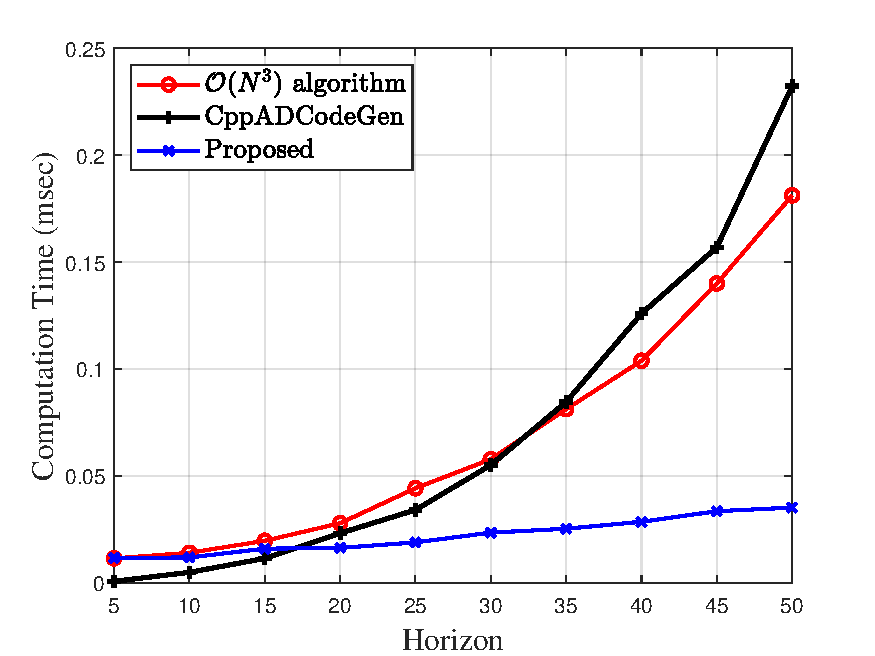
\includegraphics[width=0.8\columnwidth]{Figures/O2O3.pdf}
	\caption{Comparison of calculation times of the algorithms for Gauss-Newton Hessian approximaion with respect to the length of the Horizon.}
	\label{fig:H_O2O3}
\end{figure}


%\begin{table}
	
%	\center
	
%	\begin{tabular}{cccccc}
		
%		\hline
		
%		System & $N=20$ & $N=30$ & $N=40$ & $N=50$\\\hline
		
%		Car Parking  &  $35.4 ~\rm{sec}$ & $123.7 ~\rm{sec}$ & $351.6 ~\rm{sec}$ & $889.4 ~\rm{sec}$\\
		
%		Cart-Pole &  $59.7 ~\rm{sec}$ & $292.0 ~\rm{sec}$ & $1038.1 ~\rm{sec}$ & $2471.3 ~\rm{sec}$
		
%		\\ \hline
		
%	\end{tabular}
%	\vspace{2px}
%	\caption{Elapsed time in generation and building of a library file for $\frac{\partial \boldsymbol{\Phi}}{\partial \mathbf{U}_N}$ using CppADCodeGen.  }
%	\label{tab:elapsedtime}
%\end{table}


%\begin{table}
	
%	\center
	
%	\begin{tabular}{cccc}
		
%		\hline
		
%		System & Proposed & iLQG & ALTRO\\\hline
		
%		Car Parking ($N=100$)  &  $3.1041 (15)$ & $4.7082 (132)$ &  \\
		
%		Cart-Pole ($N=50$) &  $3597 (24)$ & $3597 (30)$ &  
		
%		\\ \hline
		
%	\end{tabular}
%	\vspace{2px}

%	\caption{The value of the objective and iteration number at the termination of algorithms. }
%	\label{tab:complexity}
%\end{table}



\subsection{Trajectory Optimization}
We tested the proposed algorithm for the trajectory optimization of different dynamic systems. Each optimization problem uses a quadratic objective and inequality constraints with upper and lower bounds on control inputs. Simulation is performed on a desktop computer with an Intel\textsuperscript{\textregistered} i7-8700 CPU running at 3.2 GHz and 32GB RAM. For performance comparison, each trajectory optimization problem is solved with SNOPT~\cite{gill2002snopt}, IPOPT~\cite{wachter2006implementation}, iLQG~\cite{6907001}, and the proposed algorithm. For SNOPT and IPOPT, functions that compute cost, analytical gradient, and constraints are written in C. The software package of iLQG is obtained from~\cite{iLQG2015}, and we converted it into a C-code for fair comparison of solve time. 
 %To compare Gauss-Newton Hessian approximation to different Hessian approximation using quasi-Newton methods, we also included Broyden–Fletcher–Goldfarb–Shanno (BFGS) algorithm~\cite{fletcher2013practical}. 
The following is a list of dynamic systems for benchmark.

\subsubsection{Cartpole} The system must perform a swing-up maneuver from randomly generated initial states while respecting control limits.

%\begin{figure}
%	\centering
%	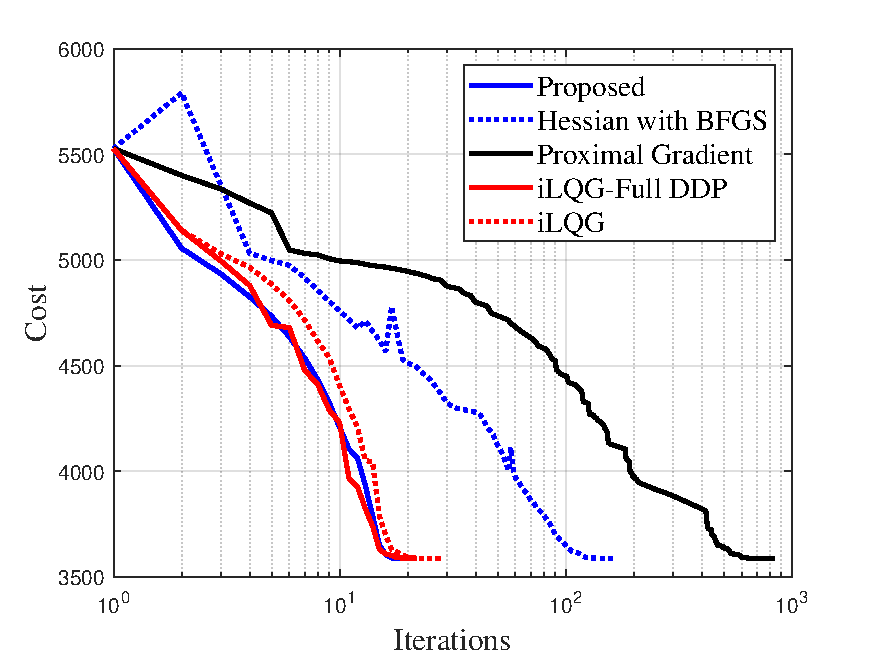
\includegraphics[width=\columnwidth]{Figures/Iteration_cartpole.pdf}
%	\caption{Cart-Pole system with $N=50$}
%	\label{fig:IT_CARTPOLE}
%\end{figure}
%\begin{figure}
%	\centering
%	\includegraphics[width=\columnwidth]{Figures/Iteration_carpark.pdf}
%	\caption{Car parking problem with $N=100$}
%	\label{fig:It_CARPARK}
%\end{figure}


%\begin{figure}
%	\centering
%	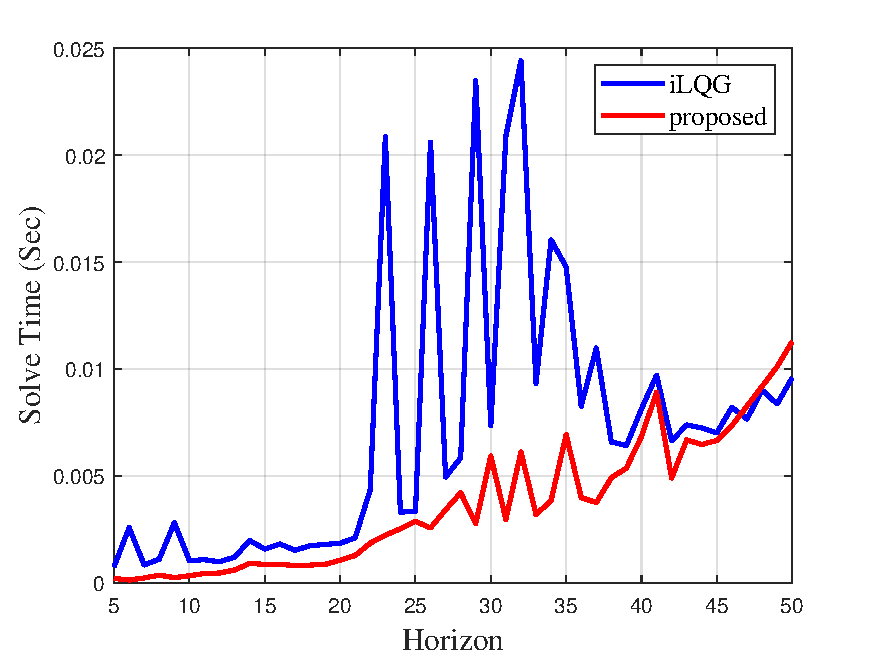
\includegraphics[width=0.8\columnwidth]{Figures/Cart_Pole_Solvetime.pdf}
%	\caption{Comparison of solve time of Cart-Pole System with respect to the Horizon Length.}
%	\label{fig:H_CARTPOLE}
%\end{figure}

\begin{figure}
	\centering
	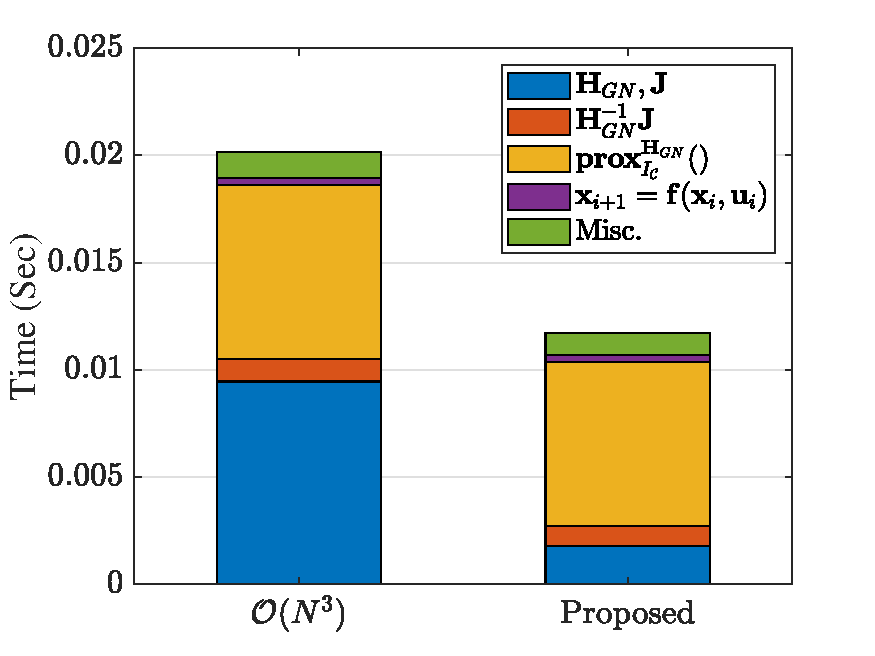
\includegraphics[width=0.7\columnwidth]{Figures/O2O3_bar.pdf}
	\caption{Breakdown of solve time for the cart-pole system with $N=50$. $\mathbf{H}_{GN}, \mathbf{J}$ are calculated with $\mathcal{O}(N^3)$ algorithm on the left and the proposed $\mathcal{O}(N^2)$ algorithm on the right. The blue area indicates required time for calculation of $\mathbf{H}_{GN}, \mathbf{J}$. }
	\label{fig:H_O2O3_bar}
\end{figure}


\begin{figure}
	\centering
\begin{subfigure}[b]{1.0\columnwidth}
	\centering
	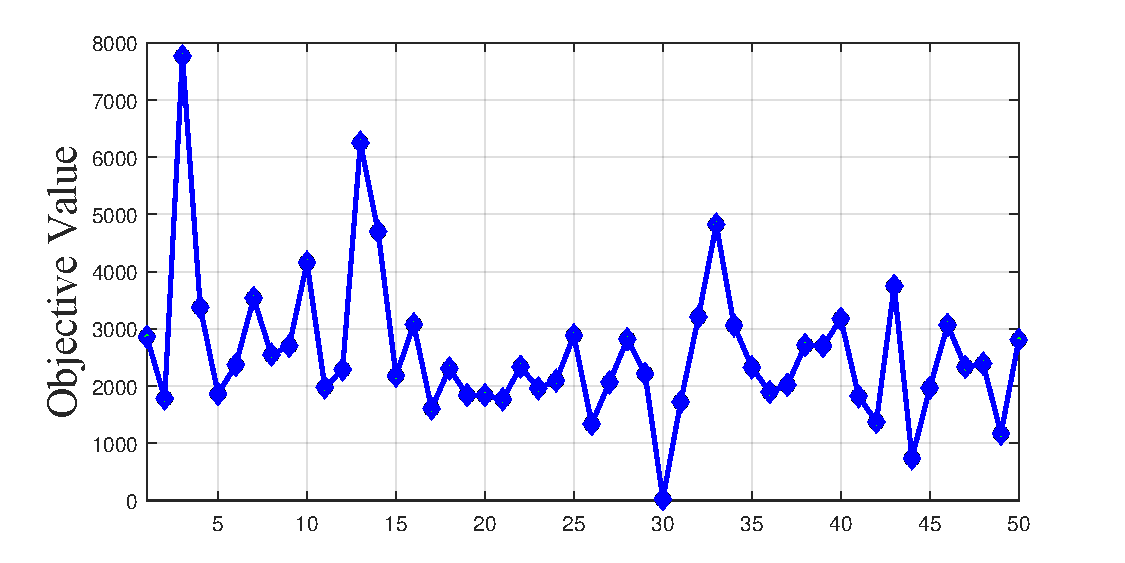
\includegraphics[width=0.9\columnwidth]{Figures/cartpole_cost_comparison10.pdf}\vskip -0.5em
	\caption{{$N=10$}}
\end{subfigure}\vskip -0.2em
\begin{subfigure}[b]{1.0\columnwidth}
	\centering
	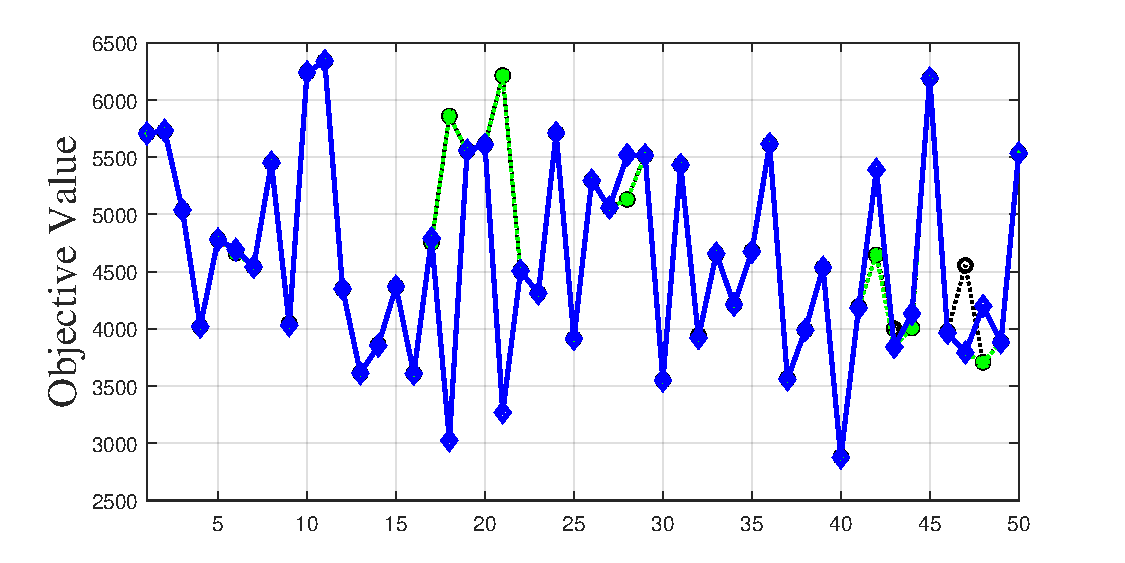
\includegraphics[width=0.9\columnwidth]{Figures/cartpole_cost_comparison50.pdf}\vskip -0.5em
	\caption{{$N=50$}}	
\end{subfigure}	\vskip -0.2em	
	\centering
	\begin{subfigure}[b]{1.0\columnwidth}
	\centering
	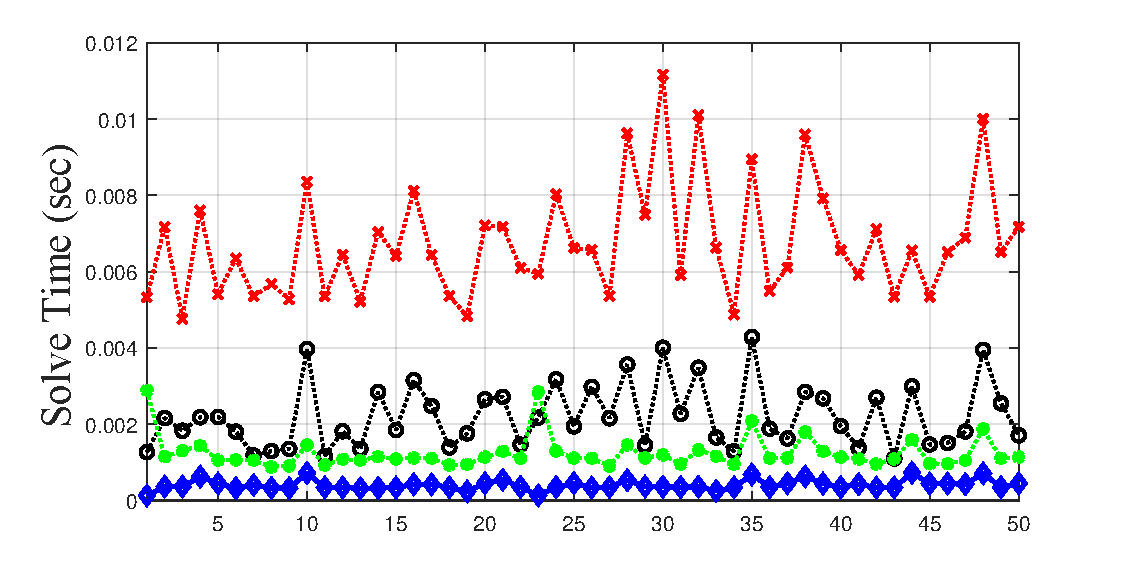
\includegraphics[width=0.9\columnwidth]{Figures/cartpole_time_comparison10.pdf}\vskip -0.5em
	\caption{{$N=10$}}	
	\end{subfigure}\vskip -0.2em
	\begin{subfigure}[b]{1.0\columnwidth}
	\centering
	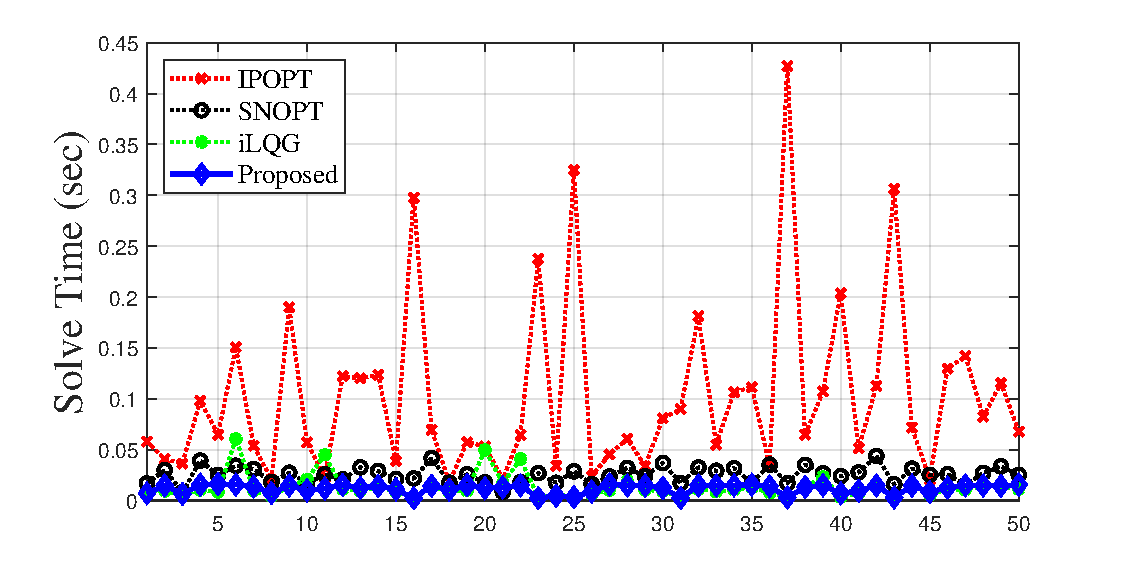
\includegraphics[width=0.9\columnwidth]{Figures/cartpole_time_comparison50.pdf}\vskip -0.5em
	\caption{{$N=50$}}	
	\end{subfigure}	\vskip -0.2em	
	\caption{Objective values and solve time  of the cart-pole system with different horizons. Each figure presents 50 problem instances with randomly generated initial states. }
	\label{fig:Car_Parking_comparison}
\end{figure}

\begin{figure}
	\centering
	\begin{subfigure}[b]{1.0\columnwidth}
		\centering
		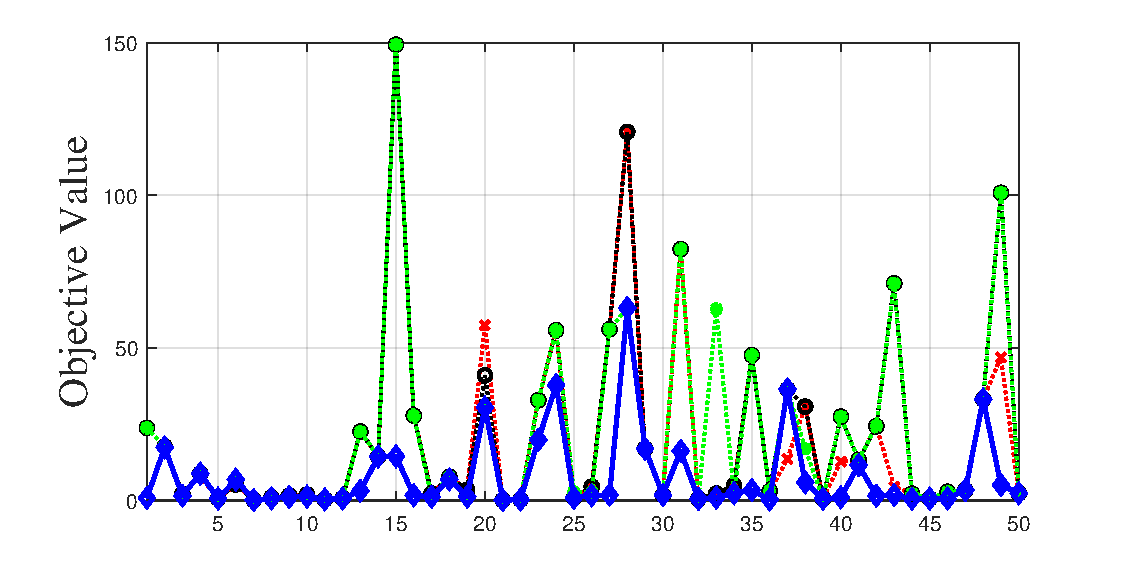
\includegraphics[width=0.9\columnwidth]{Figures/Car_Parking_cost_comparison50.pdf}\vskip -0.5em
	\caption{{$N=50$}}
	\end{subfigure}\vskip -0.2em
	\begin{subfigure}[b]{1.0\columnwidth}
		\centering
		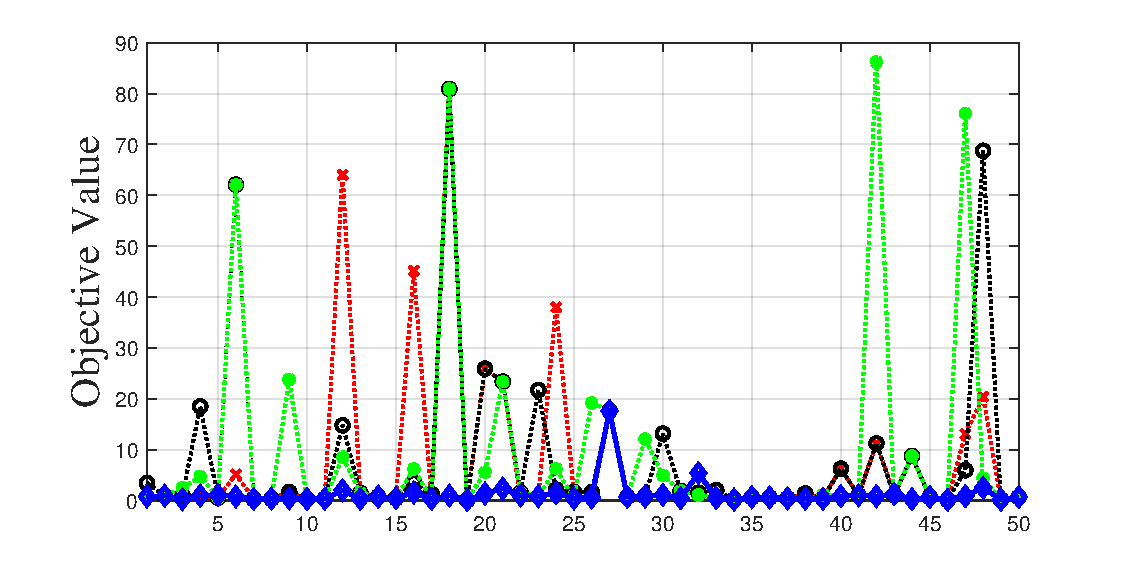
\includegraphics[width=0.9\columnwidth]{Figures/Car_Parking_cost_comparison100.pdf}\vskip -0.5em
	\caption{{$N=100$}}
	\end{subfigure}		
	\centering\vskip -0.2em
	\begin{subfigure}[b]{1.0\columnwidth}
		\centering
		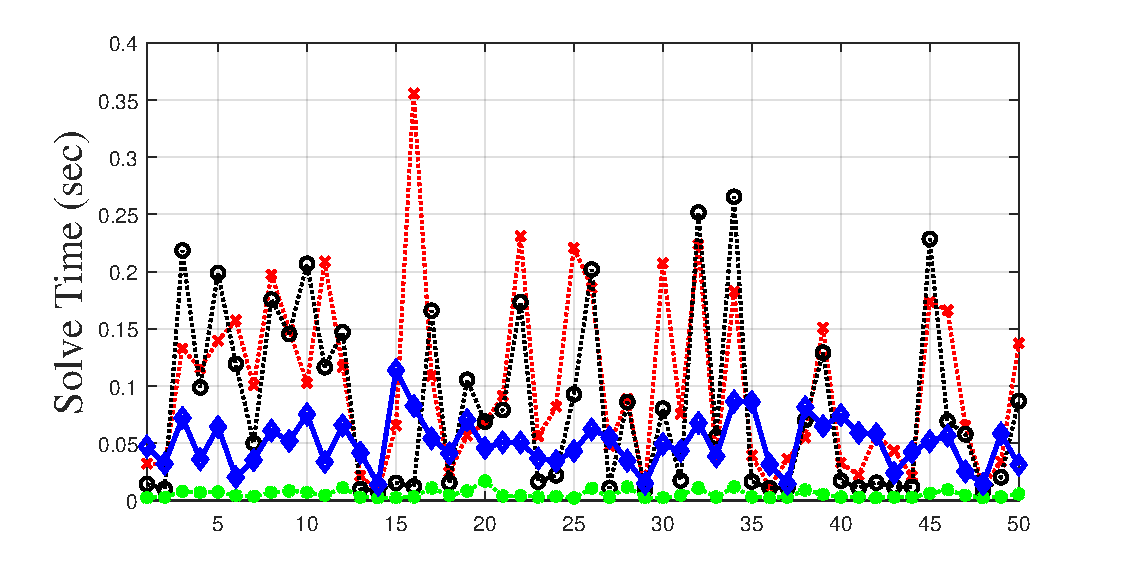
\includegraphics[width=0.9\columnwidth]{Figures/Car_Parking_time_comparison50.pdf}\vskip -0.5em
	\caption{{$N=50$}}	\end{subfigure}\vskip -0.2em
	\begin{subfigure}[b]{1.0\columnwidth}
		\centering
		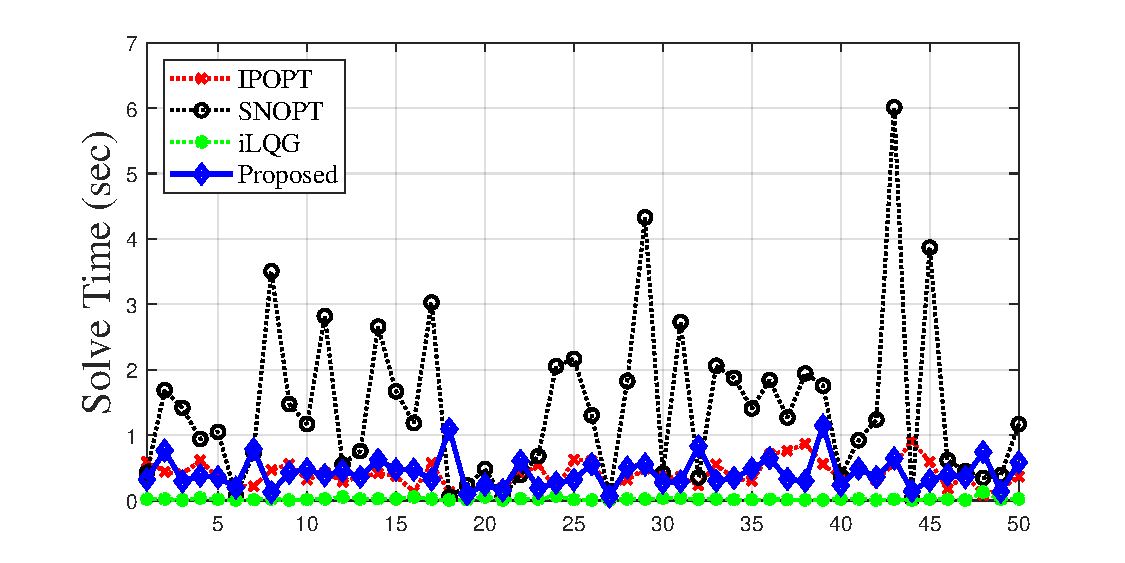
\includegraphics[width=0.9\columnwidth]{Figures/Car_Parking_time_comparison100.pdf}\vskip -0.5em
	\caption{{$N=100$}}	\end{subfigure}	\vskip -0.2em	
	\caption{Objective values and solve time of the car parking problem with different horizons. Each figure presents 50 problem instances with randomly generated initial states. }
	\label{fig:cartpole_comparison}
\end{figure}

\begin{figure}
	\centering
\vspace{-1em}
	\begin{subfigure}[b]{0.9\columnwidth}
		\centering
		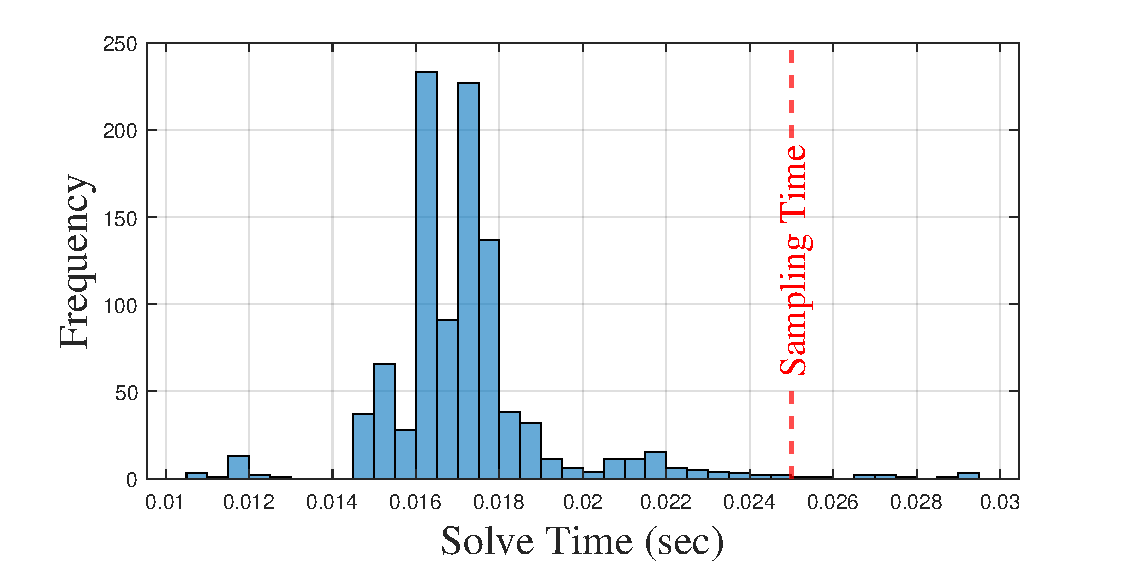
\includegraphics[width=1.0\columnwidth]{Figures/Solve_Time_Histogram_12.pdf}
	\end{subfigure}
\vskip -0.5em
	\begin{subfigure}[b]{0.9\columnwidth}
		\centering
		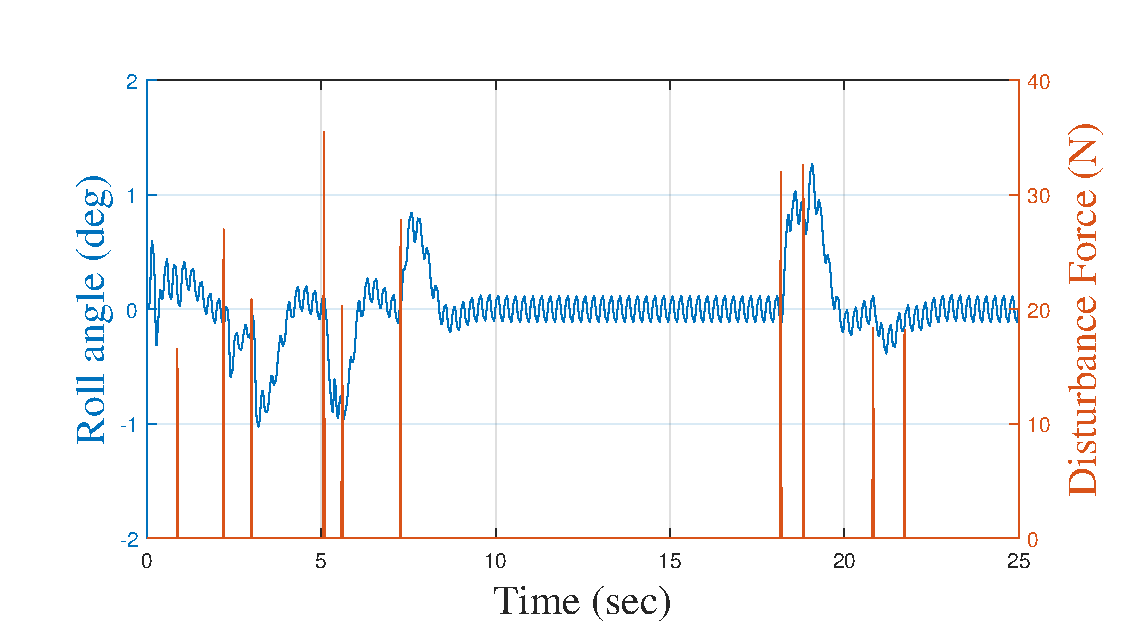
\includegraphics[width=1.0\columnwidth]{Figures/Roll_Angle_Disturbance_Force_12.pdf}
	\end{subfigure}		
	\caption{Nonlinear Model Predictive Control of a quadrupedal trotting with the speed of $1.5~\rm{m/sec}$. Random disturbance forces are applied, and their magnitude are shown in the bottom figure. Top figure displays histogram of MPC solve time during simulation.  }
	\label{fig:quadruped}
\end{figure}
%\subsubsection{Acrobat and Pendubot}
	%\vspace{-10em}

%Both are under-actuated double pendulum systems. Acrobat is limited to actuation at the “elbow” joint while Pendubot is limited to actuation at the "shoulder" joint. Both are tasked with swinging upright from the downward position.

\subsubsection{Car Parking}

The system has four states with $(x,y,\theta,v)$ where $x,y$ is the position of the car, $\theta$ is the orientation of the car, and $v$ is the velocity of the front wheels~\cite{6907001}. The two control inputs are $\omega$ the front wheel angle and $a$ the front wheel acceleration. Initially, the car is placed at random states and has to reach a desired state of $(0,0,0,0)$ at the end of the Horizon ($N=100$). 

Figure~\ref{fig:Car_Parking_comparison} shows objective values and solve time of the cart-pole system at the termination of the algorithms. In all the cases with $N=10$, the proposed algorithm provides the shortest solve time while objective values converged to the same value across the algorithms. With the larger value of $N=50$, the proposed algorithm yields on average the best objective value. However, the solve time is similar to that of iLQG.

The results of the car parking scenario are shown in Figure~\ref{fig:cartpole_comparison}. Clearly, the proposed algorithm displays the best performance in terms of the objective value significantly surpassing the other algorithms. The iLQG has the shortest solve time, but the algorithm provides values that are very far from the best ones for many cases. SNOPT and IPOPT provide objective values similar to iLQG in spite of long solve time.   


\subsection{Nonlinear Model Predictive Control}

%\subsubsection{Cartpole}

Nonlinear MPC control of a quadrupedal robot is demonstrated to validate proposed algorithm's capability to handle systems with a large number of states and control inputs. The system is modeled as a 6 DoF floating-rigid body controlled by 3 dimensional ground reaction forces at 4 legs, constituting 12 control inputs in total. This model serves as a simplified model of quadrupeds for control design and trajectory generation~\cite{8594448,8283570}. Linearized friction cone constraints are imposed on ground reaction forces as linear inequality constraints and gait sequence for the timing of stance and swing legs is imposed with equality constraints that ground reaction forces of the airborne legs should be equal to zero. The length of horizon is selected as $N=12$ with a sampling time of $0.025~\rm{sec}$. The result of trotting gait with the forward velocity of $1.5~\rm{m/sec}$ is shown in Figure~\ref{fig:quadruped}. Other types of gait such as galloping, bounding, pacing also can be controlled while handling push disturbances~\footnote{\label{note1}These results are only shown in the submitted video due to the maximum page limit}. Note that this system cannot be controlled by control-limited iLQG because of the linearized friction cone constraints.

In addition to nonlinear MPC of a quadrupedal robot, we tested our algorithm for nonlinear MPC of cart-pole, pendubot (only actuation at the "shoulder" joint), and acrobat (only actuation at the "elbow" joint) systems which are examples of nonlinear under-actuated systems~\footnoteref{note1}. 


\section{Discussion and Future Works}
\subsection{Nonlinear Constraints}
Extension of the proposed algorithm can be easily made to include more general inequality constraints although only linear inequalities are addressed in the current form of the proposed framework. Without changing the main algorithm to find $\delta \mathbf{U}$, only the proximal operator using QP solver can be replaced with the one using more general solvers such as nonlinear programming solvers to handle nonlinear constraints. This is possible due to modular structure of the proposed framework where calculation of search direction and handling of inequality constraints are carried out separately,     


\subsection{State Constraints}
Modification can be easily made to extend the proposed algorithm's functionality to handle state or mixed state-input constraints. One possible modification can come from augmented Lagrangian method that changes the objective function to the Lagrangian with additional quadratic penalty terms, and iteratively updates Lagrangian multipliers and penalty weights until convergence. %This AL method is widely used in constrained optimal control problems. For example, in~\cite{howell2019altro}, the AL method is used to propose a fast solver for constrained trajectory optimization, and the work in\cite{lantoine2012hybrid} utilizes the AL method to propose hybrid differential dynamic programming algorithm for constrained optimal control problems. 
 As application of the AL method will only change the objective function to the augmented Lagrangian without directly adding state or mixed constraints to the formulation, we predict that this modification can be done without major changes of the framework.      
\subsection{Long-Term Horizon MPC Problem}
For a long horizon MPC problem, the proposed algorithm can be numerically costly as Algorithm~\ref{alg:GNHA} has computational complexity of $\mathcal{O}(N^2)$. % and this is briefly shown in the cart-pole system when $N>47$ in Figure~\ref{fig:IT_CARTPOLE}. 
%The main reason for low numerical efficiency is caused by the process to obtain the line search direction in~\eqref{eq:GNsearchdirection} as it involves  solving QP with a large dense matrix $\mathbf{H}_{GN}$. 
 One efficient approach to find the solution of~\eqref{eq:linopt} is the iterative LQR in~\cite{1469949} utilizing discrete-time Riccati equation which has $\mathcal{O}(N)$ computational complexity. However, since this approach does not provide Gauss-Newton Hessian Approximation matrix, we have to use unscaled version of the proximal operator which could decrease the rate of convergence resulting in more iterations. %This is briefly captured in a large number of iterations of Proximal Gradient algorithm in Figure~\ref{fig:IT_CARTPOLE} and~\ref{fig:It_CARPARK}.
Therefore, there should exist a lower range of $N$ that is favorable to the proposed algorithm, and vice versa.   
	%In order to perceive information about its surrounding environment, the quadruped was outfitted with a Hokuyo UTM-30LX-EW laser range finder as shown in Fig.~\ref{fig:architecture}. This sensor provides distance data in its scan plane with an angular resolution of $0.25^\circ$. To minimize the scan time, data was collected in the sagittal plane only for angles between $45^\circ$ above the horizontal, to $90^\circ$ below the horizontal, as shown in Fig.~\ref{fig:lidarscan}. It was assumed that the motion of the robot during the scan time of $12.5$ ms had a negligible effect on the data. Pitch correction from the IMU was used to rotate this data into global coordinates.
	
	%Following each scan, a simple line segmentation algorithm was applied to detect the ground plane and the front face of the obstacle. Nguyen et al. \cite{Siegwart07} provide a thorough overview of line segmentation algorithms for planar data, and report on the promising accuracy and processing speed of the Split and Merge algorithm \cite{Horowitz74}.  In order to further decrease the computational overhead of the algorithm, a simplification of the Split and Merge algorithm, the Iterative-end-point-fit (IEPF) algorithm \cite{Ramer72} was used here.  This algorithm begins by constructing a line between the first and last points of the data. It then proceeds to take the point furtherest from the line, splits the data into two halves about this point,  and reapplies the algorithm to each half. This recursive process is repeated until all data is within a threshold distance to any segment.
	
	%To  decrease the size of the input to the IEPF algorithm, data was first preprocessed to extract a contiguous subset of points that contained the ground plane. Starting at $90^\circ$ below the horizontal, the radial distance of successive data points was monitored for a large jump above a given threshold. All data after the first jump was discarded. In addition, $(x,z)$ data in the sagittal plane within a small tolerance was clustered together and averaged to further decrease the input size. Figure \ref{fig:lidarscan} shows the preprocessed data passed to IEPF, as well as its segmented output. The long first segment in this data represents the ground plane, while the second segment represents the front face of the obstacle. 
%The distance to the second segment $d_0$ and its length  $h_0$ were then used to provide a sensed obstacle distance and height to the approach adjustment and trajectory optimization algorithms. 
%This method was found to be effective during bounding at ~3Hz despite significant pitch and small roll oscillations which perturbed the lidar scan plane, as demonstrated further in Sec.\ref{sec:results}.

%\cite{Siegwart07} - Review\\
%\cite{Ramer72} - Iterative- End-Point-Fit \\
%\cite{Horowitz74} - Split and Merge

%\begin{figure}
%\center
%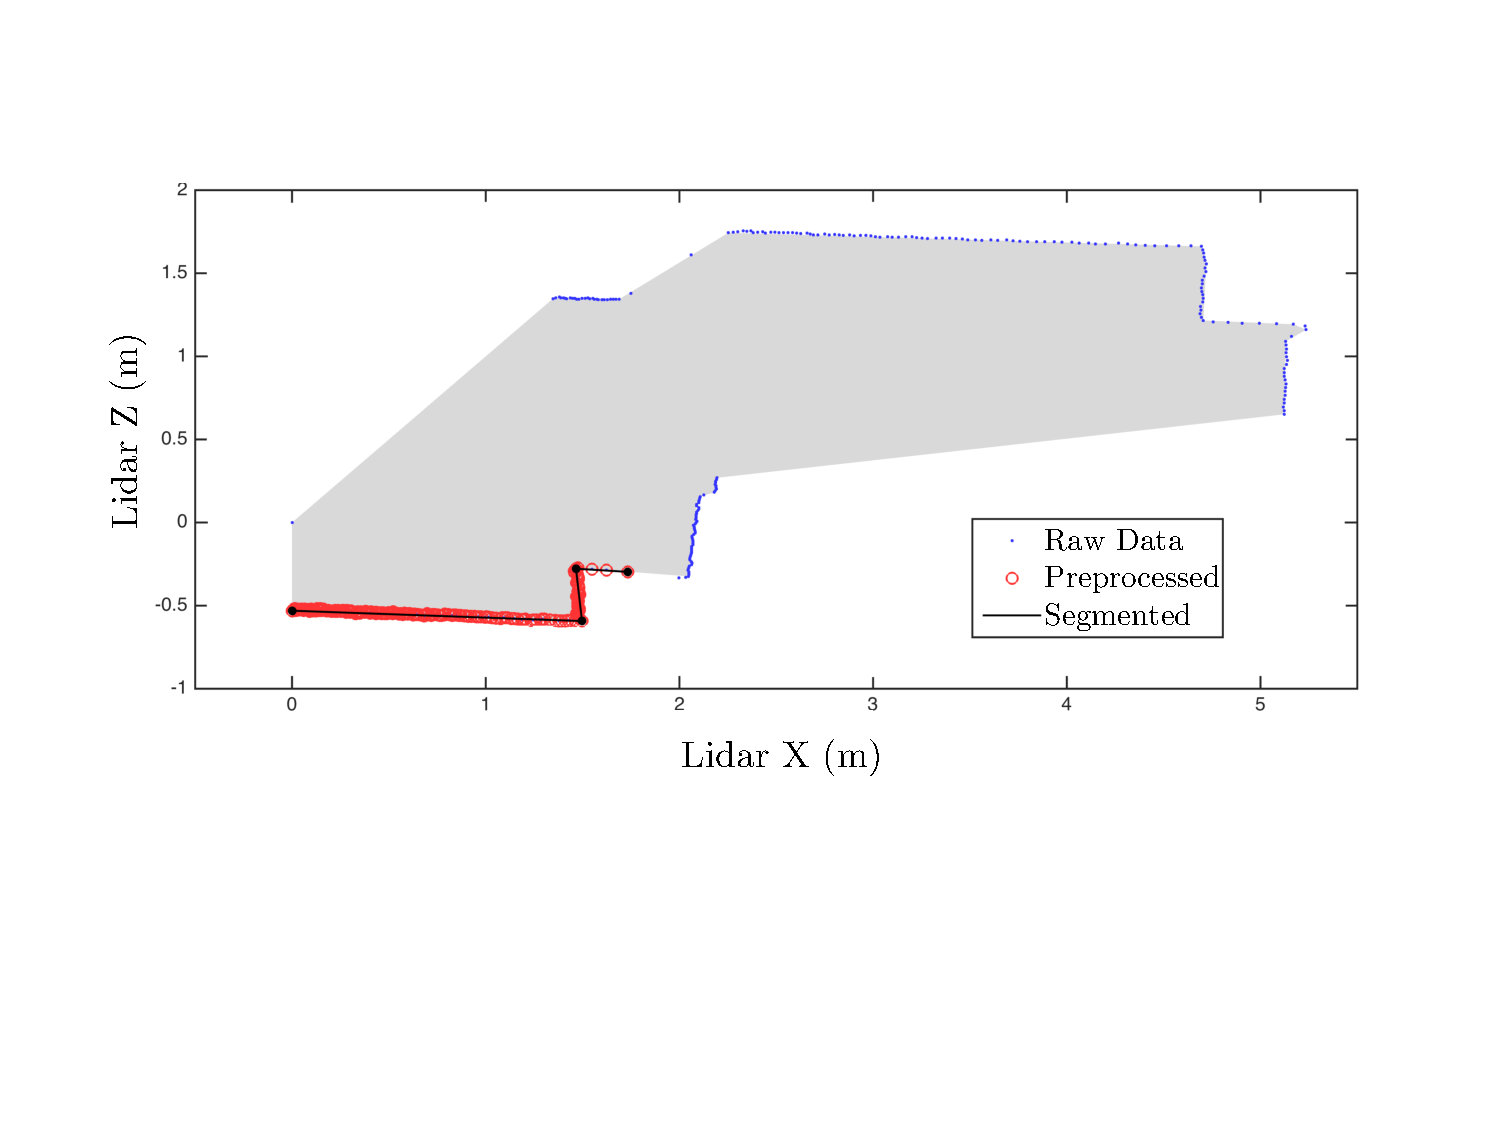
\includegraphics[width=.95\columnwidth]{Figures/HokData.pdf}
%\caption{Lidar data, preprocessing, and final segmentation for a characteristic scan over $135^\circ$ in the sagittal plane.}
%\label{fig:lidarscan}
%\end{figure}


\section{Conclusion}
We proposed a new trajectory optimization framework by combining Gauss-Newton algorithm and proximal algorithms to handle inequality constraints on controls. An efficient algorithm is also proposed for fast computation of Gauss-Newton Hessian approximation which achieved significant reduction in computational cost. Through simulation studies, we verified that the proposed algorithm has its benefit in both solve time and objective values for short  horizon MPC problems. For long horizon MPC problems, the algorithm  demonstrated reliable and robust performance providing the lowest objective values for most problem instances among the algorithms we tested  even though the solve time is higher than iLQG. 

\bibliographystyle{IEEEtran}
\bibliography{references}
\end{document}